\documentclass[twoside]{article}

\usepackage[preprint]{aistats2026}
\usepackage[utf8]{inputenc}
\usepackage[T1]{fontenc}
\usepackage[numbers,sort&compress]{natbib}
\usepackage{xcolor}
\definecolor{linkblue}{RGB}{0,90,160}

\usepackage{hyperref}
\hypersetup{
  colorlinks=true,
  citecolor=linkblue,
  linkcolor=linkblue,
  urlcolor=linkblue
}
\usepackage{booktabs}
\usepackage{adjustbox}
\usepackage{amsmath,amssymb,amsthm,amsfonts,mathtools}
\usepackage{graphicx}
\usepackage{subcaption}
\usepackage{float}
\captionsetup[subfigure]{font=footnotesize,justification=centering,singlelinecheck=false}
\usepackage{enumitem}
\usepackage{tikz}
\usetikzlibrary{arrows.meta,positioning,fit,backgrounds,shapes}
\usepackage{placeins}

\newtheorem{theorem}{Theorem}
\newtheorem{definition}{Definition}
\newtheorem{proposition}{Proposition}
\newtheorem{corollary}{Corollary}
\newtheorem{lemma}{Lemma}
\newtheorem{assumption}{Assumption}
\newtheorem{remark}{Remark}

\newcommand{\E}{\mathbb{E}}
\newcommand{\doo}{\mathrm{do}}
\newcommand{\An}{\mathrm{An}}
\newcommand{\QCBO}{\textsc{QCBO}}
\newcommand{\HQCBO}{\textsc{HQCBO}}
\newcommand{\QDCBO}{\textsc{QDCBO}}
\newcommand{\QMCBO}{\textsc{QMCBO}}
\newcommand{\CBO}{\textsc{CBO}}
\newcommand{\Gg}{\mathcal{G}}
\newcommand{\ES}{\mathbf{ES}}
\newcommand{\ESpi}{\mathbf{ES}^{\Pi}}

\definecolor{okorange}{HTML}{E69F00}
\definecolor{okblue}{HTML}{56B4E9}
\definecolor{okpurple}{HTML}{CC79A7}
\tikzset{
  obsnode/.style={circle,draw=black!75,minimum size=6.5mm,inner sep=1pt,font=\small},
  mannode/.style={obsnode,fill=okorange!45},
  tgtnode/.style={obsnode,fill=okblue!45},
  clbox/.style={draw=black!55,dashed,rounded corners,inner sep=3.2mm},
  diredge/.style={->,>=Stealth,semithick,black!80},
  bicross/.style={<->,>=Stealth,okpurple,dashdotted,semithick},
  biintra/.style={bicross},
}

\begin{document}

\runningtitle{Coarsening Confers Robustness in Causal Bayesian Optimization}
\runningauthor{Anonymous}

\twocolumn[
\aistatstitle{Coarsening Confers Robustness: \\
Causal Bayesian Optimization under Graph Misspecification}
\aistatsauthor{Anonymous}
\aistatsaddress{Anonymous}
]

\begin{abstract}
Ignore the abstract for now

We need to write this, just writing here something so that the figure appears on the right side of the page 

for visual purposes only

right 

right

right

right

right

right

right
\end{abstract}

\section{Introduction}
\label{sec:intro}

Many scientific problems require choosing interventions in complex systems: which variables to manipulate, and at what values, to optimize a target under a limited experimental budget. Bayesian optimization (BO) fits a probabilistic surrogate to costly evaluations and selects experiments sequentially. Standard BO treats the system as a black box and therefore does not use its causal structure.

Causal Bayesian optimization (CBO) \citep{agliettiCausalBayesianOptimization2020b} closes this gap by using an assumed causal graph to select intervention variables and observational data to construct prior information about their effects. Existing methods are typically presented with a directed acyclic graph (DAG); in this paper we also allow acyclic directed mixed graphs so that the supplied graph can represent latent confounding. Because causal graphs are elicited from experts or estimated from finite data, the assumed graph can be wrong. Such an error can do more than slow learning: it can exclude the best intervention from the search space.

\begin{figure}[t]
  \centering
  % Motivating example (Fig. 1): three semantic subfigures.
\begin{subfigure}[t]{0.32\linewidth}
  \centering
  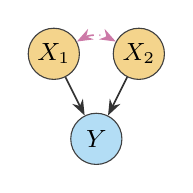
\begin{tikzpicture}[x=0.72cm,y=0.72cm]
    \node[mannode] (X1) at (0,1.15) {$X_1$};
    \node[mannode] (X2) at (1.5,1.15) {$X_2$};
    \node[tgtnode] (Y) at (0.75,-0.35) {$Y$};
    \draw[diredge] (X1) -- (Y);
    \draw[diredge] (X2) -- (Y);
    \draw[bicross] (X1) to[bend left=28] (X2);
  \end{tikzpicture}
  \caption{True graph}
  \label{fig:motivating-true}
\end{subfigure}\hfill
\begin{subfigure}[t]{0.32\linewidth}
  \centering
  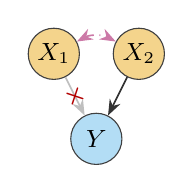
\begin{tikzpicture}[x=0.72cm,y=0.72cm]
    \node[mannode] (X1) at (0,1.15) {$X_1$};
    \node[mannode] (X2) at (1.5,1.15) {$X_2$};
    \node[tgtnode] (Y) at (0.75,-0.35) {$Y$};
    \draw[diredge,black!25] (X1) -- (Y)
      node[midway,sloped] {\textcolor{red!70!black}{\footnotesize$\boldsymbol{\times}$}};
    \draw[diredge] (X2) -- (Y);
    \draw[bicross] (X1) to[bend left=28] (X2);
  \end{tikzpicture}
  \caption{Assumed graph}
  \label{fig:motivating-assumed}
\end{subfigure}\hfill
\begin{subfigure}[t]{0.32\linewidth}
  \centering
  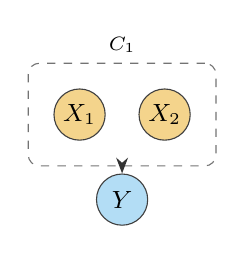
\begin{tikzpicture}[x=0.72cm,y=0.72cm]
    \node[mannode] (X1) at (0,1.15) {$X_1$};
    \node[mannode] (X2) at (1.5,1.15) {$X_2$};
    \node[tgtnode] (Y) at (0.75,-0.35) {$Y$};
    \begin{scope}[on background layer]
      \node[clbox,fit=(X1)(X2),label={[font=\scriptsize]above:$C_1$}] (C1) {};
    \end{scope}
    \draw[diredge] (C1.south) -- (Y);
  \end{tikzpicture}
  \caption{Common quotient}
  \label{fig:motivating-quotient}
\end{subfigure}

  \caption{The \textsc{ParallelParent} construction. Deleting
  $X_1\to Y$ changes the fine exploration set but not the quotient because the cluster edge $C_1\to Y$ remains through $X_2\to Y$. Orange nodes are manipulable, blue is the target, and the dash-dotted edge denotes latent
  confounding.}
  \label{fig:motivating}
\end{figure}

Figure~\ref{fig:motivating} illustrates this failure mode. The confounded parents $X_1$ and $X_2$ jointly determine $Y$, and the optimum requires setting both. If the assumed variable-level graph (the \emph{fine graph}) omits $X_1\to Y$, CBO discards every intervention containing $X_1$.

This observation motivates changing the resolution of the graph supplied to the optimizer. A partition $\Pi$ groups the variables into disjoint clusters. The resulting cluster-level directed acyclic graph (C-DAG) states relations between clusters while leaving their internal structure unspecified. In Figure~\ref{fig:motivating}(c), $X_1$ and $X_2$ form the cluster $C_1=\{X_1,X_2\}$. The edge $C_1\to Y$ survives through $X_2\to Y$, so the whole-cluster intervention remains available.

We call the resulting method quotient causal Bayesian optimization (QCBO). QCBO receives a partition and its C-DAG and restricts interventions to unions of manipulable clusters. A cluster may encode a known subsystem, policy module, or other domain-defined unit whose external relations are more reliable than its internal structure. We assume that the practitioner provides the partition and C-DAG. Coarsening removes sensitivity to hidden within-cluster distinctions, but it can also remove useful fine-grained actions. It does not protect against quotient-visible errors: deleting both parent edges in Figure~\ref{fig:motivating} removes $C_1\to Y$ and therefore changes the C-DAG consumed by QCBO.

Our contributions are fourfold:
\begin{enumerate}[leftmargin=1.5em,itemsep=2pt,topsep=2pt]
  \item We construct quotient versions of arm-based, dynamic, and model-based
  causal Bayesian optimizers, together with an adaptive refinement variant.
  \item We formalize the \emph{quotient contract}: every graph-dependent
  operation uses the supplied graph only through its quotient. This yields
  exact trajectory invariance when two fine graphs have the same quotient.
  \item We characterize the value lost by restricting interventions to
  cluster unions, prove monotonicity under refinement, and give structural
  conditions under which coarsening is lossless.
  \item Experiments isolate exploration-set and prior corruption, measure the
  action-space price, and test portability across optimizer families.
\end{enumerate}
Proofs, complete dataset graphs, and additional results appear in the appendices.

\section{Background}
\label{sec:background}
\label{sec:setup}

\subsection{Causal models and interventions}

A structural causal model (SCM) \(\mathcal M=\langle\mathbf U,\mathbf V,F,P(\mathbf U)\rangle\) consists of exogenous variables \(\mathbf U\), endogenous variables \(\mathbf V\), their structural mechanisms \(F=\{f_V:V\in\mathbf V\}\), and an exogenous distribution \(P(\mathbf U)\) \citep{pearlCausality2009}. Each endogenous variable is assigned by
\[
 V:=f_V\!\left(\operatorname{Pa}(V),\mathbf U_V\right),
\]
where \(\operatorname{Pa}(V)\) are its endogenous parents and \(\mathbf U_V\subseteq\mathbf U\) are its exogenous inputs. We write \(\operatorname{An}(V)\) for the ancestors of \(V\).

Let \(Y\in\mathbf V\) be the target and \(\mathbf X\subseteq\mathbf V\setminus\{Y\}\) the manipulable variables. An intervention consists of a nonempty set \(A\subseteq\mathbf X\) and assigned values \(a\in D(A)\), where \(D(A)\) is the intervention domain. The operator \(\doo(A=a)\) replaces the structural mechanisms of the variables in \(A\) by the constants \(a\). The resulting interventional response is
\begin{equation}
 f_A(a):=\E_{\mathcal M}[Y\mid\doo(A=a)].
 \label{eq:arm-value}
\end{equation}

A directed acyclic graph (DAG) represents the directed relations among the endogenous variables when all relevant common causes are observed. When latent common causes are present, the latent projection of the SCM is an acyclic directed mixed graph (ADMG) \(\Gg\): directed edges represent causal relations and bidirected edges represent latent confounding. Throughout, \(\Gg\) denotes the graph of the true data-generating SCM and \(\widehat{\Gg}\) denotes the graph supplied to the optimizer. Changing \(\widehat{\Gg}\) can change the optimizer's decisions, but it does not change the outcomes generated by \(\mathcal M\).

\subsection{Causal Bayesian optimization}

Causal Bayesian optimization (\CBO{}) \citep{agliettiCausalBayesianOptimization2020b} searches for an intervention that minimizes Equation~\eqref{eq:arm-value}. It maintains a Gaussian process (GP) for each retained intervention set, also called an \emph{arm}. Its exploration set consists of the graph's minimal intervention sets (MIS) \citep{leeStructuralCausalBandits}. Writing \(\widehat{\Gg}_{\bar A}\) for the graph obtained by deleting incoming edges to \(A\), this set is
\begin{equation}
 \ES(\widehat{\Gg})=\operatorname{MIS}(\widehat{\Gg})
 :=\left\{A\subseteq\mathbf X:
 \substack{A\ne\emptyset,\\
 A\subseteq\An(Y)\text{ in }\widehat{\Gg}_{\bar A}}\right\}.
 \label{eq:mis}
\end{equation}
Thus \(A\) is retained only when every intervened variable remains an ancestor of \(Y\) after the intervention removes incoming edges to \(A\).

For every retained arm, CBO places a GP prior on its response surface,
\begin{equation}
 f_A\sim\mathcal{GP}\!\left(m_A^{\widehat{\Gg}},k_A\right),
 \label{eq:cbo-gp}
\end{equation}
where \(m_A^{\widehat{\Gg}}\) and \(k_A\) are the mean and covariance functions. When the effect is identified under \(\widehat{\Gg}\), the prior mean uses an observational estimate,
\begin{equation}
 m_A^{\widehat{\Gg}}(a)
 :=\widehat{\E}_{\widehat{\Gg}}[Y\mid\doo(A=a)].
 \label{eq:causal-prior}
\end{equation}
Otherwise, our implementation uses the observational mean. Sequential interventions are selected with the base optimizer's acquisition rule; the cost-normalized expected-improvement rule and the supported causal estimators are recorded in Appendix~\ref{app:estimators}.

The supplied graph therefore affects CBO through two objects:
\[
 \widehat{\Gg}\longmapsto
 \left(\ES(\widehat{\Gg}),
 \{m_A^{\widehat{\Gg}}\}_{A\in\ES(\widehat{\Gg})}\right).
\]
A graph error can change the prior information, the available arms, or both.

\subsection{Dynamic and model-based CBO}

Dynamic causal Bayesian optimization (DCBO) \citep{agliettiDynamicCausalBayesian2021a} extends CBO to temporal causal models. It selects interventions within successive time slices while using the slice graphs and temporal transitions to transfer information over time.

Model-based causal Bayesian optimization (MCBO) \citep{sussexMODELBASEDCAUSALBAYESIAN2023} instead places GP models on the individual structural mechanisms and composes them along the causal graph. It then optimizes interventions using a GP upper confidence bound (GP-UCB) acquisition rule. These families depend on the supplied graph in different ways: DCBO through its temporal graph components and MCBO through its mechanism factorization.

\subsection{Cluster causal graphs}

Let \(\Pi\) be a partition of \(\mathbf V\), and let \(\chi:\mathbf V\to\Pi\) map each variable to its unique cluster. The quotient graph \(\Gg^\Pi\) has a directed edge \(\chi(u)\to\chi(v)\) whenever \(u\to v\) is present in \(\Gg\) and \(\chi(u)\ne\chi(v)\); bidirected edges are mapped analogously. The quotient is a cluster-level causal graph, or C-DAG. A partition is \emph{valid} when the directed part of its quotient is acyclic \citep{madaleno2026a}.

A C-DAG preserves which causal and confounding relations exist between clusters while leaving within-cluster structure unspecified. C-DAG identification is sound and complete over the fine graphs represented by the quotient \citep{CausalEffectIdentification}. This established identification layer is the input to the optimizers introduced next.

\section{Quotient causal optimizers}
\label{sec:methods}

Each quotient optimizer replaces only the graph-dependent components of its base method. It receives a partition and a valid supplied C-DAG and otherwise retains the base method's acquisition and update rules.

\subsection{Arm-based quotient CBO}

Quotient causal Bayesian optimization (\QCBO{}) receives the partition \(\Pi\), supplied C-DAG \(\widehat{\Gg}^{\Pi}\), target \(Y\), observational data, and intervention domains. We take every nonmanipulable variable, including \(Y\), to be a singleton cluster. Hence a cluster that contains a manipulable variable contains only manipulable variables. Let
\[
 \Pi_M:=\{C\in\Pi:C\subseteq\mathbf X\}
\]
be the manipulable clusters, let \(C_Y:=\chi(Y)\) be the target cluster, and let \(U_\Pi(S):=\bigcup_{C\in S}C\) expand a set of clusters to its variables. QCBO applies the MIS rule to the C-DAG:
\begin{equation}
 \ESpi(\widehat{\Gg}^{\Pi})
 :=\left\{U_\Pi(S):
 \substack{\emptyset\ne S\subseteq\Pi_M,\\
 S\subseteq\An(C_Y)\text{ in }
 (\widehat{\Gg}^{\Pi})_{\bar S}}\right\}.
 \label{eq:qcbo-arms}
\end{equation}
Every retained arm therefore intervenes on complete clusters.

For each arm \(A\in\ESpi(\widehat{\Gg}^{\Pi})\), a complete causal-effect identification procedure determines whether the observational distribution identifies its prior mean. The resulting two-tier prior is
\begin{equation}
 m_A^\Pi(a)=
 \begin{cases}
  \widehat{\E}[Y\mid\doo(A=a)] & \text{if identified},\\
  \bar Y_{\mathrm{obs}} & \text{otherwise.}
 \end{cases}
 \label{eq:two-tier-prior}
\end{equation}
Non-identifiable effects start from the observational mean and are learned from interventions.

\begin{assumption}[Estimator boundary]
The supplied partition is valid. The identification test is complete, while the numerical implementation is sound for the supported backdoor, frontdoor, and \(g\)-computation functionals but is not complete. An identified functional outside this implemented class receives the observational-mean prior.
\end{assumption}

As a sanity check, the singleton partition recovers the fine graph, the CBO exploration set, and the CBO prior construction arm by arm. A formal statement and proof appear in Appendix~\ref{app:proofs}.

\subsection{Dynamic and model-based quotient variants}

Quotient dynamic CBO (\QDCBO{}) replaces every DCBO time-slice graph and its temporal transitions by their quotients. It selects cluster-union interventions within each slice and otherwise retains DCBO's temporal acquisition and update logic.

Quotient model-based CBO (\QMCBO{}) replaces MCBO's node mechanisms by joint conditional cluster mechanisms
\[
 P(\mathbf X_C\mid\mathbf X_{\operatorname{pa}(C)}),
\]
and composes them along the C-DAG. Here \(\operatorname{pa}(C)\) denotes the parent clusters of \(C\). Joint rather than marginal mechanisms preserve dependence among variables within a cluster.

An SCM is \emph{causally sufficient} when every common cause of its endogenous variables is represented in the model, so its causal graph has no bidirected edges. Under causal sufficiency and a valid partition, the joint cluster factorization is sound for whole-cluster interventions. It does not determine effects of interventions on strict subsets of a cluster; two fine models can agree on every quotient-level input and disagree on such a sub-cluster effect. Appendix~\ref{app:proofs} states and proves both facts.

\begin{center}
\small
\adjustbox{max width=\linewidth}{%
\begin{tabular}{@{}ll@{}}
\toprule
Family & Graph-dependent quotient object \\
\midrule
CBO \(\to\) QCBO & intervention arms and causal priors \\
DCBO \(\to\) QDCBO & time-slice graphs and transitions \\
MCBO \(\to\) QMCBO & joint cluster mechanisms \\
\bottomrule
\end{tabular}}
\end{center}

\subsection{Adaptive refinement}

Hierarchical quotient CBO (\HQCBO{}) begins from a coarse partition and a declared refinement hierarchy. When its plateau rule detects stalled progress, it splits clusters participating in the incumbent. It rejects a split if the resulting directed quotient is cyclic, retains data for arms that remain available, and initializes only newly exposed arms. The plateau rule and hierarchy are heuristic inputs: refinement is not guaranteed to expose a useful fine-grained intervention. Section~\ref{sec:refinement} states the conditional recovery and invariance guarantees.

\section{Robustness and the price of coarsening}
\label{sec:theory}

\subsection{Quotient invariance}
\label{sec:invariance}

For a graph \(G\) and partition \(\Pi\), define the quotient input
\begin{equation}
 Q_\Pi(G):=(\Pi,G^\Pi).
 \label{eq:quotient}
\end{equation}
For a complete run, let
\[
 \xi:=(\mathcal M,\mathcal D_0,\omega,\eta)
\]
collect the fixed true SCM, initial data, optimizer random stream, and hyperparameters. The true SCM belongs to the environment rather than the optimizer's input. Let \(\tau_{\mathcal A}(\widehat{\Gg},\xi)\) denote the complete trajectory of optimizer \(\mathcal A\): its selected arms, intervention values, observations, and incumbents.

An optimizer satisfies the \emph{quotient contract} when every graph-dependent operation uses \(\widehat{\Gg}\) only through \(Q_\Pi(\widehat{\Gg})\). For a true graph \(\Gg\), define the protected class
\begin{equation}
 E_\Pi(\Gg):=
 \{\widehat{\Gg}\text{ ADMG over }\mathbf V:
 Q_\Pi(\widehat{\Gg})=Q_\Pi(\Gg)\}.
 \label{eq:protected-class}
\end{equation}
Within-cluster edits and quotient-redundant cross-cluster edits remain in this class. An edit that adds or removes a quotient edge does not.

\begin{proposition}[Exact quotient invariance]
\label{prop:contract}
At fixed \(\xi\), every optimizer satisfying the quotient contract obeys
\[
 Q_\Pi(\widehat{\Gg})=Q_\Pi(\widehat{\Gg}')
 \quad\Longrightarrow\quad
 \tau_{\mathcal A}(\widehat{\Gg},\xi)
 =\tau_{\mathcal A}(\widehat{\Gg}',\xi).
\]
\end{proposition}

Equal quotient inputs give equal first decisions. The fixed true SCM then gives the coupled runs equal observations, so induction yields identical subsequent decisions and observations. In Figure~\ref{fig:motivating}, deleting \(X_1\to Y\) is protected because \(X_2\to Y\) preserves the quotient edge. Deleting both parent edges is quotient-visible and is not protected.

\begin{corollary}[Portability of the quotient contract]
\label{cor:portability}
QCBO and QMCBO satisfy Proposition~\ref{prop:contract}; QDCBO satisfies it within every time slice. At the singleton partition, QCBO, QDCBO, and QMCBO reduce to CBO, DCBO, and MCBO, respectively.
\end{corollary}

The converse characterization---trajectory invariance over every protected class implies factorization through \(Q_\Pi\)---is stated in Appendix~\ref{app:proofs}.

\subsection{Price of restricting interventions}
\label{sec:price}

The action family allowed by \(\Pi\) consists of nonempty unions of manipulable clusters:
\begin{equation}
 \mathcal U(\Pi):=
 \left\{\bigcup_{C\in S}C:
 \emptyset\ne S\subseteq\Pi_M\right\}.
 \label{eq:cluster-actions}
\end{equation}
For an intervention set \(A\), define its best population value by
\[
 \mu^\star(A):=\min_{a\in D(A)}f_A(a).
\]
Let \(\Pi_{\mathrm{fine}}:=\{\{v\}:v\in\mathbf V\}\) denote the singleton partition. The best value reachable at resolution \(\Pi\) and its loss relative to the fine action space are
\begin{equation}
 V(\Pi):=\min_{A\in\mathcal U(\Pi)}\mu^\star(A),
 \qquad
 \Delta(\Pi):=V(\Pi)-V(\Pi_{\mathrm{fine}}).
 \label{eq:price}
\end{equation}
We call \(\Delta(\Pi)\ge0\) the \emph{price of coarsening}.

A partition \(\Pi'\) \emph{refines} \(\Pi\), written \(\Pi'\preceq\Pi\), when every cluster of \(\Pi'\) is contained in a cluster of \(\Pi\). Refinement exposes additional interventions.

\begin{proposition}[Monotonicity and price of coarsening]
\label{prop:price}
For valid \(\Pi'\preceq\Pi\),
\[
 \mathcal U(\Pi)\subseteq\mathcal U(\Pi'),
 \qquad
 0\le\Delta(\Pi')\le\Delta(\Pi).
\]
Moreover,
\[
 \Delta(\Pi)=0
 \iff
 \arg\min_{A\in\mathcal U(\Pi_{\mathrm{fine}})}\mu^\star(A)
 \cap\mathcal U(\Pi)\ne\emptyset.
\]
\end{proposition}

Thus coarsening is lossless exactly when at least one fine-optimal intervention is a union of clusters. The MIS-reduction result in Appendix~\ref{app:proofs} connects this action-family value to the quotient exploration set. Even when \(\Delta(\Pi)=0\), a partition can change arm count, intervention dimension, cost, and finite-budget behavior.

\subsection{Protected-class regret separation}
\label{sec:separation}

Let \(\hat z_t=(\hat A_t,\hat a_t)\) be the incumbent intervention after trial \(t\), and define its population value by
\[
 \mu(\hat z_t):=\E_{\mathcal M}
 [Y\mid\doo(\hat A_t=\hat a_t)].
\]
With \(y^\star:=V(\Pi_{\mathrm{fine}})\), define instantaneous and cumulative incumbent regret by
\begin{equation}
 r_t:=\mu(\hat z_t)-y^\star,
 \qquad
 R_T:=\sum_{t=1}^{T}r_t.
 \label{eq:regret}
\end{equation}

Fix a true SCM \(\mathcal M\) with graph \(\Gg\), while the optimizer receives a hypothesis graph \(\widehat{\Gg}\). Let \(R_T(\mathcal A,\widehat{\Gg})\) denote regret at fixed \(\xi\), and define worst-case regret over the protected class by
\[
 R_T^{\mathrm{wc}}(\mathcal A,\Pi,\Gg)
 :=\sup_{\widehat{\Gg}\in E_\Pi(\Gg)}
 R_T(\mathcal A,\widehat{\Gg}).
\]
For a cluster-union incumbent,
\begin{equation}
 \mu(\hat z_t)-y^\star
 =\underbrace{V(\Pi)-y^\star}_{\text{coarsening price}}
 +\underbrace{\mu(\hat z_t)-V(\Pi)}_{\text{optimization error}}.
 \label{eq:regret-decomposition}
\end{equation}

A \emph{semi-Markovian SCM} has mutually independent exogenous variables, each of which is a parent of at most two endogenous variables; shared exogenous parents represent the bidirected edges of its latent-projection ADMG.

\begin{theorem}[Protected-class regret separation]
\label{thm:separation}
The following statements hold.
\begin{enumerate}[label=(\roman*),leftmargin=1.6em,itemsep=2pt,topsep=2pt]
 \item For every \(\beta>0\), there exist a semi-Markovian SCM, a valid
 partition with \(\Delta(\Pi)=0\), and a hypothesis
 \(\widehat{\Gg}\in E_\Pi(\Gg)\) obtained by deleting one directed edge, such
 that every optimizer whose initial and sequential interventions lie in
 \(\operatorname{MIS}(\widehat{\Gg})\) and whose incumbent is selected among
 executed interventions satisfies
 \[
  r_t\ge\beta\quad\text{for every }t,
  \qquad
  R_T^{\mathrm{wc}}(\mathcal A,\Pi,\Gg)\ge\beta T.
 \]
\item If an optimizer satisfies Proposition~\ref{prop:contract}, executes only cluster-union interventions, and selects its incumbent among executed actions, then its trajectory is identical for every \(\widehat{\Gg}\in E_\Pi(\Gg)\) and
 \[
 \begin{aligned}
 R_T^{\mathrm{wc}}(\mathcal A,\Pi,\Gg)
 &=R_T(\mathcal A,\Gg)\\
 &=T\Delta(\Pi)
 +\sum_{t=1}^{T}\bigl(\mu(\hat z_t)-V(\Pi)\bigr).
 \end{aligned}
 \]
\end{enumerate}
\end{theorem}

Part (i) is instantiated by the exploration-set corruption experiment in Section~\ref{sec:exp-a}: a quotient-invisible edge deletion can force linear regret even when coarsening is lossless. Part (ii) separates the unavoidable structural price from optimization error within the quotient action space.

\subsection{When coarsening is lossless}
\label{sec:zero-price}

For a fine intervention \(A\subseteq\mathbf X\), define its \emph{cluster completion}
\[
 A^\Pi:=\bigcup\{C\in\Pi:C\cap A\ne\emptyset\}.
\]
This is the smallest cluster-union intervention containing \(A\).

\begin{definition}[Full intervention support]
\label{def:full-support}
A partition has full intervention support when, after any fine intervention \(\doo(A=a)\), every natural value attainable by the additional variables in \(A^\Pi\setminus A\) is also permitted when completing the intervention to \(A^\Pi\).
\end{definition}

\begin{definition}[Cluster-contained confounding]
\label{def:ccc}
Represent a semi-Markovian SCM by a nonparametric structural equation model with mutually independent exogenous variables. A partition has cluster-contained confounding when, for every \(A\subseteq\mathbf X\), the exogenous ancestors of the naturally responding variables \(A^\Pi\setminus A\) after \(\doo(A)\) are disjoint from the exogenous ancestors of \(Y\) after \(\doo(A^\Pi)\).
\end{definition}

\begin{corollary}[Graphical zero-price condition]
\label{cor:zero-price}
In a semi-Markovian SCM, full intervention support and cluster-contained confounding imply
\[
 V(\Pi)=V(\Pi_{\mathrm{fine}})
 \qquad\text{and}\qquad
 \Delta(\Pi)=0.
\]
\end{corollary}

These conditions are sufficient but not necessary. The practitioner-facing assumption is the structural placement of confounding. Appendix~\ref{app:proofs} introduces the potential-outcome notation needed to derive the corresponding cross-world independence statement and prove the corollary.

\subsection{Fixed partitions and refinement}
\label{sec:refinement}

\begin{proposition}[Linear regret floor]
\label{prop:floor}
For a fixed partition,
\[
 r_t\ge\Delta(\Pi)\quad\text{for every }t,
 \qquad
 R_T\ge T\Delta(\Pi).
\]
\end{proposition}

A positive coarsening price therefore creates a regret floor that no learning within the fixed action space can remove. The adaptive method of Section~\ref{sec:methods} can remove it only by visiting a sufficiently fine partition.

\begin{definition}[Incumbent consistency]
\label{def:consistency}
The base optimizer is incumbent-consistent on the action space of a partition \(\Pi_J\) if continued optimization on that space satisfies \(\mu(\hat z_t)\to V(\Pi_J)\) almost surely.
\end{definition}

\begin{corollary}[Conditional refinement recovery]
\label{cor:recovery}
If the refinement schedule visits a valid partition \(\Pi_J\) with \(\Delta(\Pi_J)=0\) and the base optimizer is incumbent-consistent on that action space, then
\[
 r_t\longrightarrow0,
 \qquad
 R_T/T\longrightarrow0.
\]
\end{corollary}

\begin{corollary}[Adaptive refinement invariance]
\label{cor:adaptive-invariance}
Let \(\tau_{\mathcal H}\) denote the HQCBO trajectory under a declared hierarchy \(\mathcal H\). If the visited partitions are \(\Pi_0,\ldots,\Pi_J\), then
\[
 \left[\forall j,\ \Gg^{\Pi_j}=(\Gg')^{\Pi_j}\right]
 \Longrightarrow
 \tau_{\mathcal H}(\Gg)=\tau_{\mathcal H}(\Gg').
\]
\end{corollary}

Recovery is conditional on the hierarchy exposing a lossless partition, the heuristic trigger reaching it, and the base optimizer being incumbent-consistent. Refinement can also reveal previously hidden graph errors, so validity must be checked after every split.
\section{Experiments}
\label{sec:experiments}

\subsection{Evaluation design and datasets}
\label{sec:exp-design}

The evaluation separates four claims: robustness to exploration-set corruption, robustness to causal-prior corruption, the action-space price of coarsening, and portability of the quotient contract. Table~\ref{tab:experiment-map} summarizes this design. In every misspecification comparison, the true SCM, initial data, hyperparameters, and random stream are paired. Only the graph supplied to the optimizer changes.

The controlled suite uses three SCMs with closed-form population effects: \textsc{ParallelParent}, \textsc{FrontDoor}, and \textsc{MediatedChain}. Their fine graphs, partitions, and quotients appear in Appendix~\ref{app:dags}. Each SCM provides one shared observational dataset; the optimizer receives its first $n_{\mathrm{obs}}=100$ observations. All displayed disturbance variables in this suite are mutually independent standard Gaussians; shared latent variables induce the stated bidirected edges. Interventional outcomes, including the initial design, are evaluated using the exact population expectation $\E[Y\mid\doo(A=a)]$. We use $30$ paired seeds, three initial intervention points per arm, unit cost per intervened variable, and $T=50$ trials, increased to $60$ for \textsc{MediatedChain}.

The portability suite follows each base method's released protocol. The CBO family contains ToyGraph, CompleteGraph (``Synthetic''), and SimplifiedCoralGraph, with $10$ seeds, $n_{\mathrm{obs}}=100$, ten initial points per arm, $40$ trials, and minimization. The Coral simulator is the linear structural equation model (SEM) benchmark introduced by \citet{agliettiCausalBayesianOptimization2020b}: its graph is based on a Bermuda reef ecosystem model and its mechanisms were fit to $50$ field observations. The DCBO family uses stationary, independent, and nonstationary synthetic temporal SEMs, with $20$ seeds, three time slices, ten trials per slice, and minimization. The MCBO family uses its ToyGraph and PSAGraph simulators with $20$ seeds, $T=100$, GP-UCB exploration parameter $\beta=10$, zero observation noise, and maximization. PSAGraph is the model-based harness's adaptation of the prostate-specific-antigen simulator used in the original CBO study.

We report four complementary quantities: the best-so-far population objective, cumulative incumbent regret for the controlled minimization experiments, paired trajectory deviation for testing exact invariance, and the final objective value with its standard error across seeds. The \emph{best-so-far population value} evaluates the incumbent in the true SCM. For the controlled minimization suite, \emph{cumulative incumbent regret} is Equation~\eqref{eq:regret}. \emph{Paired trajectory deviation} compares the selected arms, intervention values, and incumbents of coupled correct- and wrong-graph runs. For the portability suite we report the final value as mean $\pm$ standard error.

\begin{table*}[t]
\centering
\caption{Evaluation map. Arrow up for maximization and down for minimization objective give the objective direction.}
\label{tab:experiment-map}
\small
\adjustbox{max width=\textwidth}{%
\begin{tabular}{@{}lllllll@{}}
\toprule
Study & Data & Perturbation & Comparison & Objective & Primary metric & Purpose \\
\midrule
A & \textsc{ParallelParent} & delete $X_1\to Y$ & CBO versus QCBO & $\downarrow$ & regret; deviation & exploration-set robustness \\
B & \textsc{FrontDoor} & add $X_1\leftrightarrow M$ & CBO versus QCBO & $\downarrow$ & regret; deviation & prior robustness \\
C & \textsc{MediatedChain} & refine $\{X_1,X_2\}$ & CBO, QCBO, HQCBO & $\downarrow$ & value; regret & price and recovery \\
D & eight family tasks & quotient graph view & base versus quotient & $\downarrow/\uparrow$ & final objective value & portability \\
\bottomrule
\end{tabular}}
\end{table*}

\subsection{Exploration-set corruption}
\label{sec:exp-a}

The \textsc{ParallelParent} SCM is shown in Figure~\ref{fig:motivating} and Appendix~\ref{app:dags}. Its structural equations are
\begin{equation}
 \begin{aligned}
 U&=0.4\varepsilon_0,\\ X_1&=U+0.3\varepsilon_1,\\
 X_2&=U+0.3\varepsilon_2,\\
 Y&=(X_1-2)^2+(X_2+2)^2
  +0.1\varepsilon_Y.
 \end{aligned}
 \label{eq:parallel-parent-scm}
\end{equation}
Under the correct graph, the fine MIS are $\{X_1\}$, $\{X_2\}$, and $\{X_1,X_2\}$, and the joint arm attains $y^\star=0$ at $(2,-2)$. Deleting $X_1\to Y$ from the hypothesis graph removes every arm containing $X_1$ and leaves only $\{X_2\}$. Its exact population optimum is $4.25$, so no amount of optimization under the wrong fine graph can close this gap.

After $50$ trials, correct-graph CBO reaches $0.0016\pm0.0002$, whereas misspecified CBO ends at $4.2500\pm0.0000$ (mean $\pm$ standard error). Their cumulative incumbent regrets are $4.21\pm0.37$ and $216.23\pm1.12$, respectively. The latter value is close to the structural lower bound $4.25T=212.5$; the excess is finite-budget optimization error within the misspecified action space.

For $\Pi=\{\{X_1,X_2\},\{Y\}\}$, the same deletion is invisible because $X_2\to Y$ preserves the quotient edge. The paired QCBO runs select the same arms and intervention values at every trial, and their incumbent trajectories have zero deviation. Figure~\ref{fig:minimal-misspec}(a) therefore separates a permanent fine-graph arm exclusion from exact quotient invariance. A quotient-visible $X_1\leftrightarrow Y$ perturbation serves as the negative control and changes the QCBO trajectory, with maximum paired incumbent deviation $21.45$.

\subsection{Prior corruption without arm loss}
\label{sec:exp-b}

The \textsc{FrontDoor} graph in Appendix~\ref{app:dags} contains $X_1\to M\to Y$ and latent $X_1\leftrightarrow Y$. Its SCM is
\begin{equation}
 \begin{aligned}
 U&=0.4\varepsilon_0,\\ X_1&=U+0.3\varepsilon_1,\\
 M&=2X_1+0.2\varepsilon_M,\\
 Y&=2\!\left[1-\exp\!\left\{-\frac{(M-1)^2}{2(0.3)^2}\right\}\right]+U+0.1\varepsilon_Y.
 \end{aligned}
 \label{eq:frontdoor-scm}
\end{equation}
Its population objective is minimized by $\doo(M=1)$. Under the correct graph, $\doo(M)$ is identified by adjustment for $X_1$ and $\doo(X_1)$ by the frontdoor criterion. Adding a spurious $X_1\leftrightarrow M$ leaves the fine MIS unchanged but makes both prior means non-identifiable. This design therefore changes the prior while holding the available arms fixed.

Fine CBO loses its observational head start and accumulates additional regret while searching for the narrow optimum, but it can recover from interventional observations because the optimal arm remains available. The paired increase in cumulative regret is $5.91\pm1.04$ at $T=50$; the final values are $0.0003\pm0.0003$ under the correct graph and $0.0035\pm0.0022$ under the corrupted graph. This is a transient finite-budget effect rather than an action-space exclusion like in \ref{sec:exp-a}. The perturbation is internal to $\{X_1,M\}$ and disappears in the quotient, so the paired QCBO decisions and incumbent trajectories are identical. The right panel of Figure~\ref{fig:minimal-misspec} contrasts this transient fine-graph effect with exact quotient invariance.

\begin{figure}[t]
  \centering
  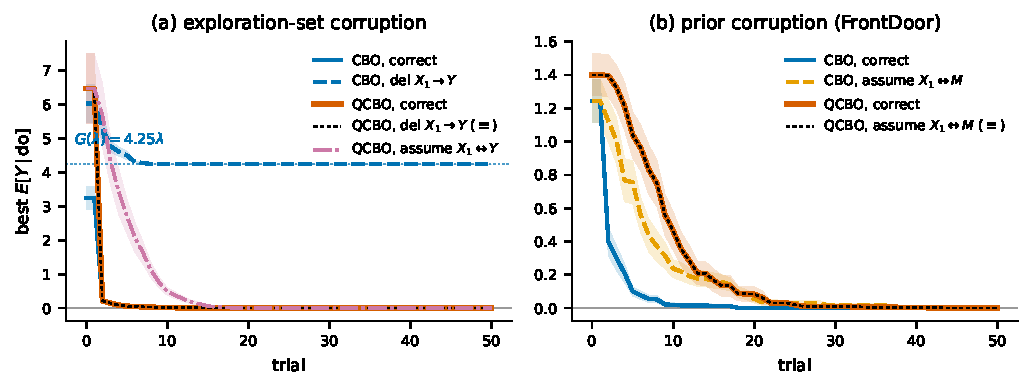
\includegraphics[width=0.90\linewidth]{figures/minimal_misspec}
  \caption{Correct and misspecified trajectories, mean $\pm$ standard error over $30$ seeds. Top: deleting $X_1\to Y$ removes the optimal fine arm, whereas QCBO is unchanged because the edit is invisible in the quotient. Bottom: corruption of an identified prior slows fine CBO, whereas QCBO remains exactly invariant.}
  \label{fig:minimal-misspec}
\end{figure}

\subsection{Action-space price and refinement}
\label{sec:exp-c}

The \textsc{MediatedChain}, in Appendix~\ref{app:dags}, graph has $X_1\to X_2\to Y$, with
\[
  X_2=2X_1+\varepsilon_2,
  \qquad
  Y=(X_2-4)^2+\varepsilon_Y.
\]
Fine CBO can execute $\doo(X_1=2)$ without intervening on $X_2$. The edge $X_1\to X_2$ therefore remains active, giving
\[
\begin{aligned}
  X_2&=4+\varepsilon_2,\\
  \E[Y\mid\doo(X_1=2)]
  &amp;=
  \operatorname{Var}(\varepsilon_2)
  =
  0.04.
\end{aligned}
\]

Fixed QCBO cannot execute $\doo(X_1)$ alone because $X_1$ and $X_2$ belong to the same manipulable cluster. Its only arm intervenes jointly:
\[
  \doo(X_1=x_1,X_2=x_2).
\]
Intervening on $X_2$ removes the edge $X_1\to X_2$, so $x_1$ no longer affects the target. Since the intervention domain restricts $x_2\in[-2,2]$, the best permitted value is
\[
  \min_{x_2\in[-2,2]}(x_2-4)^2=4.
\]
Hence
\[
  V(\Pi)=4,
  \qquad
  y^\star=0.04,
  \qquad
  \Delta(\Pi)=3.96.
\]

Consequently, every fixed-QCBO incumbent has instantaneous regret at least $3.96$, and Proposition~\ref{prop:floor} gives the permanent lower bound $R_T\ge3.96T$. Fine CBO does not incur this floor because its MIS retains $\{X_1\}$. HQCBO removes it only after the declared hierarchy splits $\{X_1,X_2\}$ and exposes the singleton arm. Figure~\ref{fig:minimal-refine} shows the resulting best-value and cumulative-regret trajectories. CBO, fixed QCBO, and HQCBO finish at $0.0400\pm0.0000$, $4.0000\pm0.0000$, and $0.0400\pm0.0000$, with cumulative regrets $5.46\pm1.61$, $243.23\pm0.90$, and $36.97\pm1.18$, respectively. HQCBO refines at trial $7.4\pm0.1$; all $30$ declared splits are accepted. The fixed-QCBO result exceeds the theoretical floor $60\times3.96=237.6$ only by its within-space optimization error. The experiment demonstrates recovery for this declared split; it does not imply that the plateau rule always selects a useful refinement.

\begin{figure}[t]
  \centering
  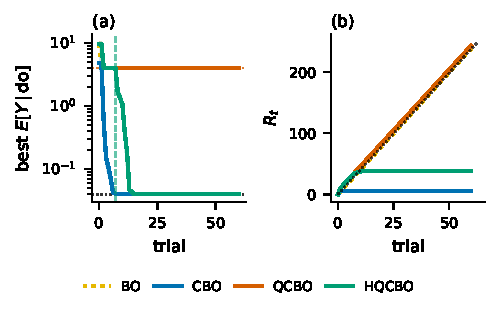
\includegraphics[width=0.90\linewidth]{figures/minimal_refine}
  \caption{Best-so-far population objective on
  \textsc{MediatedChain}, mean $\pm$ standard error over $30$ seeds.
  Fixed QCBO cannot execute $\doo(X_1)$; refinement exposes this arm.}
  \label{fig:minimal-refine}
\end{figure}

\subsection{Portability across optimizer families}
\label{sec:exp-d}

\begin{figure*}[t]
  \centering
  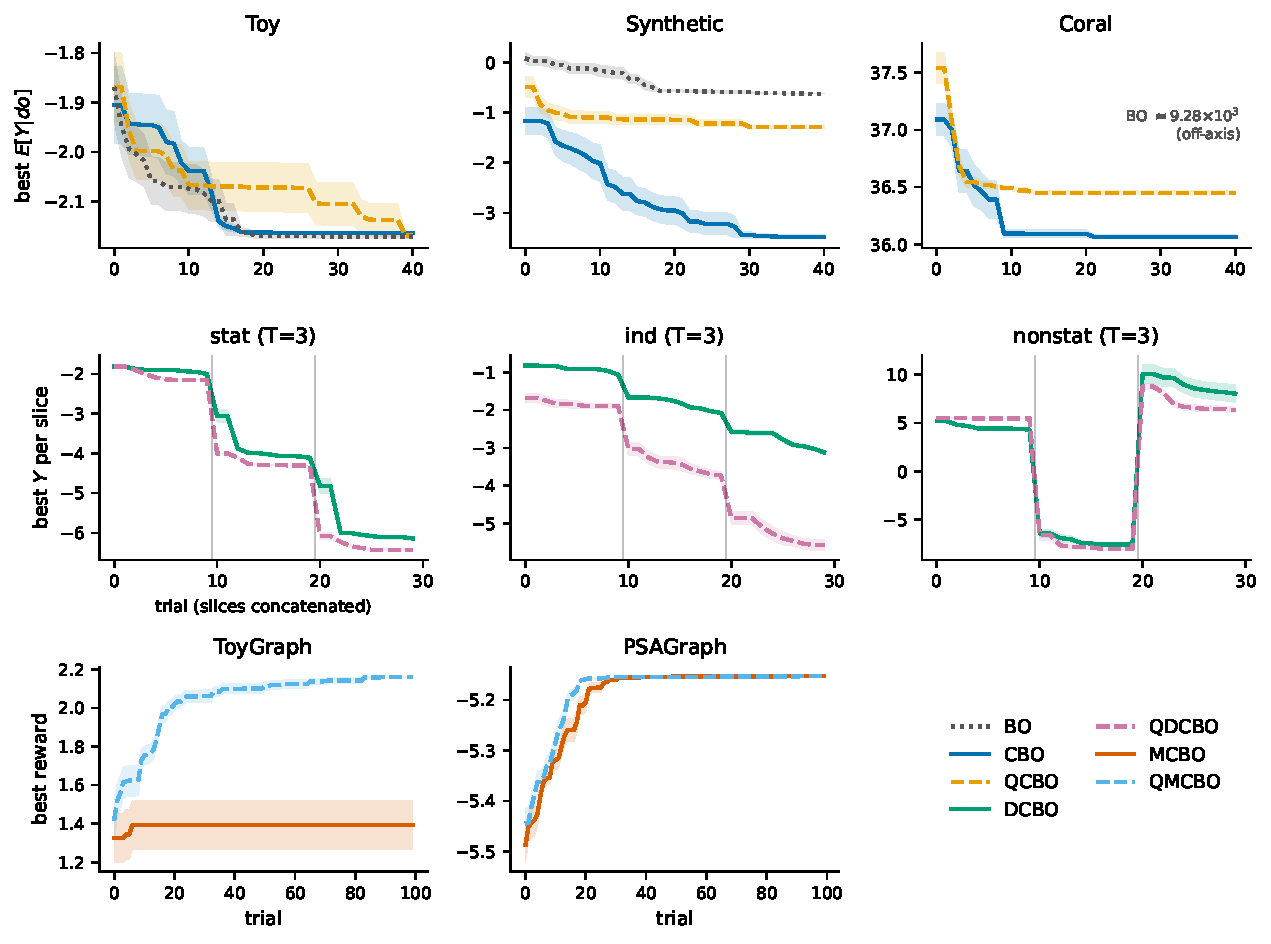
\includegraphics[width=\linewidth]{figures/family_suite}
  \captionsetup{width=\linewidth}
  \caption{Quotient methods and their corresponding base methods under the
  released family protocols, reported as mean $\pm$ standard error.
  Top: CBO minimization. Middle: dynamic minimization over three time
  slices. Bottom: MCBO maximization.}
  % TODO(author): validate the unresolved MCBO result before submission.
  \label{fig:family-suite}
\end{figure*}

Figure~\ref{fig:family-suite} compares each quotient construction with its base optimizer on the eight tasks described above; all corresponding DAGs and C-DAGs are in Appendix~\ref{app:dags}. The structural prediction is exact: QDCBO is invariant in all $60$ paired dynamic runs and QMCBO in all $40$ paired model-based runs, whereas their base methods change under the same graph-view perturbations. This confirms that the quotient contract is independent of the family-specific acquisition and surrogate construction.

Table~\ref{tab:family-finals} gives the final population value and paired quotient disadvantage for each task. For $\downarrow$ rows the paired difference is quotient minus base; for $\uparrow$ rows it is base minus quotient. Positive values therefore always mean that the quotient ended worse. 

\begin{table}[t]
  \centering
  \caption{Final objective value, reported as mean $\pm$ standard error
  across seeds. The arrows indicate the optimization direction:
  $\downarrow$ denotes minimization and $\uparrow$ maximization.}
  \label{tab:family-finals}
  \small
  \setlength{\tabcolsep}{5pt}
  \begin{tabular}{@{}lcc@{}}
    \toprule
    \textbf{Task} & \textbf{Base final} & \textbf{Quotient final} \\
    \midrule

    \multicolumn{3}{@{}l}{%
      \textit{CBO vs. QCBO ($n=10$ seeds)}} \\
    Toy $\downarrow$
      & $-2.16 \pm 0.00$ & $-2.13 \pm 0.03$ \\
    Synthetic $\downarrow$
      & $-3.14 \pm 0.19$ & $-1.25 \pm 0.07$ \\
    Coral $\downarrow$
      & $36.08 \pm 0.02$ & $36.42 \pm 0.01$ \\

    \addlinespace[3pt]
    \multicolumn{3}{@{}l}{%
      \textit{DCBO vs. QDCBO ($3$ time slices; $n=20$ seeds)}} \\
    Stationary $\downarrow$
      & $-6.14 \pm 0.05$ & $-6.43 \pm 0.02$ \\
    Independent $\downarrow$
      & $-3.12 \pm 0.06$ & $-5.57 \pm 0.15$ \\
    Nonstationary $\downarrow$
      & $8.03 \pm 0.90$ & $6.33 \pm 0.29$ \\

    \addlinespace[3pt]
    \multicolumn{3}{@{}l}{%
      \textit{MCBO vs. QMCBO ($n=20$ seeds)}} \\
    ToyGraph $\uparrow$
      & $1.39 \pm 0.13$ & $2.16 \pm 0.00$ \\
    PSAGraph $\uparrow$
      & $-5.15 \pm 0.00$ & $-5.15 \pm 0.00$ \\
    \bottomrule
  \end{tabular}
\end{table}

\section{Related work}
\label{sec:related}

Graph-agnostic and causal entropy optimization methods learn over candidate graphs online \citep{mukherjeeGraphAgnosticCausal2024,branchiniCausalEntropyOptimization2023}, while causal-bandit guarantees price learning an unknown graph within the horizon \citep{luCausalBanditsUnknown2021}. Our setting instead studies commitment to a fixed coarse input. These approaches are complementary: a graph learner could operate over, or trigger refinement of, a quotient.

The construction builds on cluster-DAG identification \citep{CausalEffectIdentification} and is related to causal abstraction and macro-level structure learning \citep{beckersAbstractingCausalModels2019,madaleno2026a}. We coarsen manipulable inputs and explicitly characterize the actions removed by that choice.

\section{Discussion and limitations}
\label{sec:limitations}

Exact invariance requires the correct quotient; quotient-visible errors and incorrect partitions remain harmful. The zero-price condition is sufficient and structural, and its cross-world consequence is not directly testable from single-world data. Refinement is heuristic, with recovery conditional on visiting a lossless partition and on consistency of the base optimizer. Different partitions also induce different arm counts, initialization costs, and intervention costs. Finally, QMCBO inherits the causal-sufficiency assumption of its model-based factorization.

\section{Conclusion}
\label{sec:conclusion}

Coarsening makes precisely those graph distinctions that disappear in the quotient irrelevant to optimization. Within the resulting protected class, the complete trajectory is invariant. The price is the optimal value of fine interventions excluded by the partition, which is monotone under refinement and zero under the stated structural conditions. Theoretical and empirical results show that using quotients can prevent catastrophic graph errors, while hierarchical refinement provides a conditional route back to the fine action space.

\bibliographystyle{abbrvnat}
\bibliography{references}

\appendix \onecolumn \raggedbottom

\section{Proofs and additional technical results}
\label{app:proofs}

\subsection{Method-specific results}

\begin{proposition}[Identity recovery]
\label{prop:identity}
At \(\Pi=\Pi_{\mathrm{fine}}\), the quotient graph equals the fine graph, the QCBO exploration set equals \(\operatorname{MIS}(\widehat{\Gg})\), and its prior construction coincides arm by arm with CBO. QDCBO and QMCBO likewise reduce to DCBO and MCBO.
\end{proposition}

\begin{proof}
At the singleton partition, \(\chi\) is one-to-one and quotienting changes no edge. Unions of manipulable singleton clusters are exactly the subsets of \(\mathbf X\), so Equation~\eqref{eq:qcbo-arms} is Equation~\eqref{eq:mis}. The C-DAG identification queries are then the same queries used by CBO. The dynamic slice graphs and model-based joint cluster mechanisms also reduce to their node-level counterparts.
\end{proof}

\begin{proposition}[Soundness of joint cluster mechanisms]
\label{prop:cluster-soundness}
Under causal sufficiency and a valid partition, every intervention on a union of clusters \(S\) satisfies
\[
 P(\mathbf V\mid\doo(\mathbf x_S))
 =\prod_{C\notin S}
 P(\mathbf X_C\mid\mathbf X_{\operatorname{pa}(C)})
 \big|_{\mathbf X_S=\mathbf x_S}.
\]
\end{proposition}

\begin{proof}
Apply the fine truncated factorization and group its factors by clusters. Within a cluster, the chain rule combines the member-level factors into the joint conditional mechanism. Validity orders the resulting mechanisms along the C-DAG. The joint conditional is essential: replacing it by a product of member-level marginals would discard within-cluster dependence.
\end{proof}

\begin{proposition}[Sub-cluster effects are not identified by cluster mechanisms]
\label{prop:qexposure}
There exist two causally sufficient SCMs with the same valid quotient, joint cluster mechanisms, and whole-cluster interventional distributions, but different values of \(P(Y\mid\doo(A=a))\) for a strict subset \(A\) of a cluster.
\end{proposition}

\begin{proof}
Let \(C=\{X_2,X_3\}\) be a root cluster and \(Y=X_2+\varepsilon_Y\). In one SCM take \(X_2=\varepsilon_2\) and \(X_3=cX_2+\varepsilon_3\); in another, choose the reverse linear-Gaussian factorization of the same joint distribution. The models agree on the joint law of \(C\) and every whole-cluster intervention. Under \(\doo(X_3=x)\), however, \(X_2\) remains mean zero in the first model and changes linearly with \(x\) in the second. Quotient-level inputs therefore do not identify the sub-cluster effect.
\end{proof}

\subsection{Quotient invariance}

\begin{proof}[Proof of Proposition~\ref{prop:contract}]
Write the run as decisions \(d_1,d_2,\ldots\) and datasets \(\mathcal D_0,\mathcal D_1,\ldots\), with
\[
 d_t=f_t\!\left(
 Q_\Pi(\widehat{\Gg}),\mathcal D_{t-1},\omega_t,\eta
 \right).
\]
Equal quotients, initial data, random streams, and hyperparameters imply equal first decisions. The fixed true SCM produces the same coupled observation, so the updated datasets also agree. Induction gives equality of every decision, observation, incumbent, and stopping event.
\end{proof}

\begin{proof}[Proof of Corollary~\ref{cor:portability}]
By construction, QCBO's arm set and prior means depend on the supplied graph only through its C-DAG. QDCBO applies the same replacement within each time slice, and QMCBO composes only the joint mechanisms indexed by its C-DAG. Each construction therefore satisfies the quotient contract. Identity recovery follows from Proposition~\ref{prop:identity}.
\end{proof}

\begin{proposition}[Necessity of the quotient contract]
\label{prop:converse}
If, for every ADMG \(\Gg\), the trajectory map is constant on \(E_\Pi(\Gg)\) at fixed \(\xi\), then it factors through \(Q_\Pi\).
\end{proposition}

\begin{proof}
For each quotient \(q\), define \(\bar\tau(q)\) as the common trajectory produced by any \(\widehat{\Gg}\) satisfying \(Q_\Pi(\widehat{\Gg})=q\). Constancy over each protected class makes this definition independent of the representative. Hence
\[
 \tau(\widehat{\Gg})
 =\bar\tau\!\left(Q_\Pi(\widehat{\Gg})\right).
\]
\end{proof}

\subsection{Price and protected-class separation}

\begin{lemma}[MIS reduction]
\label{lem:mis-reduction}
Let \(\mathcal G\) be an ADMG with manipulable variables \(\mathbf X\) and target \(Y\). For \(A\subseteq\mathbf X\), define
\[
 A':=A\cap\An_{\mathcal G_{\bar A}}(Y).
\]
Then:
\begin{enumerate}[label=(\roman*)]
 \item for every \(a\in D(A)\),
 \[
  P(Y\mid\doo(A=a))
  =P\!\left(Y\mid\doo(A'=a|_{A'})\right);
 \]
\item if \(A'\ne\varnothing\), then \(A'\in\operatorname{MIS}(\mathcal G)\); \item consequently, optimizing over \(\{\varnothing\}\cup\operatorname{MIS}(\mathcal G)\) attains the same population optimum as optimizing over all subsets of \(\mathbf X\).
\end{enumerate}
\end{lemma}

\begin{proof}
Set \(R:=A\setminus A'\). Suppose that some \(r\in R\) has a directed path to \(Y\) in \(\mathcal G_{\bar A'}\). This path cannot enter \(A'\). Let \(r^\star\) be the last member of \(R\) on the path. The subpath from \(r^\star\) to \(Y\) contains no further member of \(A\), so it also exists in \(\mathcal G_{\bar A}\). This contradicts \(r^\star\notin\An_{\mathcal G_{\bar A}}(Y)\). Thus, while \(A'\) remains intervened on, variables in \(R\) cannot causally affect \(Y\), proving (i).

For every \(v\in A'\), a directed path from \(v\) to \(Y\) in \(\mathcal G_{\bar A}\) cannot enter another member of \(A\). It therefore also exists in \(\mathcal G_{\bar A'}\), proving (ii). Applying (i) and (ii) to every candidate intervention proves (iii).
\end{proof}

Consequently, when the null intervention is handled consistently, the best value over quotient MIS expanded to fine variables equals the best value over the corresponding cluster-union action family.

\begin{proof}[Proof of Proposition~\ref{prop:price}]
Every union of clusters in \(\Pi\) is a union of clusters in a refinement \(\Pi'\), and every such union is available at the singleton partition. The population minima are therefore over nested action families:
\[
 V(\Pi_{\mathrm{fine}})\le V(\Pi')\le V(\Pi).
\]
Equality between the first and last terms holds exactly when a fine-optimal intervention belongs to \(\mathcal U(\Pi)\).
\end{proof}

\begin{proof}[Proof of Theorem~\ref{thm:separation}]
For part (i), use \textsc{ParallelParent} with manipulable variables \(\{X_1,X_2\}\), domains \([-3,3]^2\), edges \(X_1\to Y\) and \(X_2\to Y\), latent \(X_1\leftrightarrow X_2\), and partition \(\{\{X_1,X_2\},\{Y\}\}\). Choose the objective curvature so that the best \(\{X_2\}\)-only intervention has value \(\beta\), while the joint arm attains \(y^\star=0\). Deleting \(X_1\to Y\) preserves the quotient through \(X_2\to Y\) but leaves \(\operatorname{MIS}(\widehat{\Gg})=\{\{X_2\}\}\). Every executed intervention and eligible incumbent therefore has regret at least \(\beta\), giving \(R_T\ge\beta T\). The whole-cluster arm remains globally optimal, so \(\Delta(\Pi)=0\).

For part (ii), Proposition~\ref{prop:contract} makes the trajectory and regret constant over \(E_\Pi(\Gg)\). Adding and subtracting \(V(\Pi)\) gives
\[
 r_t=\Delta(\Pi)+\mu(\hat z_t)-V(\Pi).
\]
The second term is nonnegative because every incumbent is an executed cluster-union action. Summing over \(t\) gives the stated decomposition.
\end{proof}

\subsection{Lossless coarsening}

For the exact bridge used in this subsection, fix \(A\subseteq\mathbf X\) and \(a\in D(A)\). Let
\[
 B:=A^\Pi\setminus A
\]
be the variables added by cluster completion. Under \(\doo(A=a)\), let \(B(a)\) denote their natural response and \(Y(a)\) the target response. Under \(\doo(A=a,B=b)\), let \(Y(a,b)\) denote the target response, and define
\[
 D_B(a):=\{b:(a,b)\in D(A^\Pi)\}.
\]

\begin{proposition}[Sufficient potential-outcome conditions for zero price]
\label{prop:free}
If, for every \(A\subseteq\mathbf X\) and \(a\in D(A)\),
\[
 \operatorname{supp}(B(a))\subseteq D_B(a)
 \quad\text{and}\quad
 B(a)\perp Y(a,b)\quad\text{for every }b\in D_B(a),
\]
then \(V(\Pi)=V(\Pi_{\mathrm{fine}})\) and \(\Delta(\Pi)=0\).
\end{proposition}

\begin{proof}
Consistency and the stated independence give
\[
\begin{aligned}
 \E[Y(a)]
 &=\int \E[Y(a,b)\mid B(a)=b]\,\mathrm dP_{B(a)}(b)\\
 &=\int \E[Y(a,b)]\,\mathrm dP_{B(a)}(b)\\
 &\ge \inf_{b\in D_B(a)}\E[Y(a,b)],
\end{aligned}
\]
where support inclusion justifies the final inequality. Thus \(\mu^\star(A^\Pi)\le\mu^\star(A)\). Taking minima and using \(\mathcal U(\Pi)\subseteq\mathcal U(\Pi_{\mathrm{fine}})\) gives equality.
\end{proof}

\begin{lemma}[Cluster containment implies cross-world independence]
\label{lem:ccc}
In the nonparametric structural equation representation of Definition~\ref{def:ccc}, let \(\mathbf U_B(A)\) be the exogenous ancestors of \(A^\Pi\setminus A\) after \(\doo(A)\), and let \(\mathbf U_Y(A)\) be the exogenous ancestors of \(Y\) after \(\doo(A^\Pi)\). Cluster-contained confounding implies
\[
 B(a)\perp Y(a,b)
\]
for every \(A\), \(a\), and \(b\in D_B(a)\).
\end{lemma}

\begin{proof}
Recursive substitution writes
\[
 B(a)=f_B\bigl(\mathbf U_B(A);a\bigr),
 \qquad
 Y(a,b)=f_Y\bigl(\mathbf U_Y(A);a,b\bigr).
\]
Cluster-contained confounding requires \(\mathbf U_B(A)\cap\mathbf U_Y(A)=\emptyset\). Because the exogenous variables are mutually independent, functions of the two disjoint sets are independent.
\end{proof}

\begin{proof}[Proof of Corollary~\ref{cor:zero-price}]
Full intervention support gives \(\operatorname{supp}(B(a))\subseteq D_B(a)\), while Lemma~\ref{lem:ccc} gives \(B(a)\perp Y(a,b)\). Proposition~\ref{prop:free} then applies.
\end{proof}

\begin{remark}[Cross-world premise]
The independence \(B(a)\perp Y(a,b)\) is not testable from a single observational or interventional distribution. It is not imposed as a primitive assumption in Corollary~\ref{cor:zero-price}; it is derived from the structural condition in Definition~\ref{def:ccc}.
\end{remark}

\subsection{Refinement results}

\begin{proposition}[Refinement can invalidate a quotient]
\label{prop:refinement-validity}
There exist a valid partition \(\Pi\) and a refinement \(\Pi'\preceq\Pi\) for which \(\Gg^\Pi\) is acyclic but \(\Gg^{\Pi'}\) contains a directed cycle. Validity must therefore be checked after every split.
\end{proposition}

\begin{proof}
Let the fine graph contain \(a_1\to b_1\) and \(b_2\to a_2\). The single cluster \(\{a_1,a_2,b_1,b_2\}\) has an acyclic one-node quotient. Refining it into \(\{a_1,a_2\}\) and \(\{b_1,b_2\}\) exposes both quotient directions and produces a two-cycle.
\end{proof}

\begin{proof}[Proof of Proposition~\ref{prop:floor}]
Every incumbent belongs to the fixed action family, so \(\mu(\hat z_t)\ge V(\Pi)\). Subtracting \(y^\star=V(\Pi_{\mathrm{fine}})\) gives \(r_t\ge\Delta(\Pi)\); summing gives the cumulative bound.
\end{proof}

\begin{proof}[Proof of Corollary~\ref{cor:recovery}]
At a visited lossless partition, incumbent consistency gives \(\mu(\hat z_t)\to V(\Pi_J)=y^\star\), hence \(r_t\to0\) almost surely. Because \(R_T/T\) is the arithmetic mean of \(r_1,\ldots,r_T\), this also implies \(R_T/T\to0\).
\end{proof}

\begin{proof}[Proof of Corollary~\ref{cor:adaptive-invariance}]
Proceed by induction over refinement phases. Within phase \(j\), all graph-dependent behavior factors through \((\Pi_j,\Gg^{\Pi_j})\). Equal quotients and equal trajectory prefixes therefore produce the same phase trajectory, plateau decision, and next split. Repeating through \(\Pi_J\) proves equality of the adaptive trajectories.
\end{proof}
\clearpage
\section{Acquisition and numerical estimation}
\label{app:estimators}

\subsection{Acquisition rules}

After $t$ evaluations of arm $A$, let $\mu_{A,t}(a)$ and $\sigma_{A,t}(a)$ be its GP posterior mean and standard deviation, and let $y_t^{\mathrm{best}}$ be the best observed interventional outcome. For minimization, expected improvement is
\[
 \operatorname{EI}_{A,t}(a)
 :=\E\!\left[
 \bigl(y_t^{\mathrm{best}}-f_A(a)\bigr)_+
 \mid\mathcal D_t\right].
\]
The arm-based implementation selects an arm and value maximizing $\operatorname{EI}_{A,t}(a)/c(A,a)$, where $c(A,a)$ is the intervention cost. Model-based experiments retain their base method's lower confidence bound for minimization, or upper confidence bound for maximization,
\[
 \mu_{A,t}(a)\mp\sqrt{\beta_t}\,\sigma_{A,t}(a),
\]
where $\beta_t>0$ controls exploration.

\subsection{Causal-effect estimation}

The complete identification check is performed on the ADMG supplied to the optimizer. When a query is identified, the returned functional is instantiated using the supported plug-in estimators.

For a valid backdoor set $Z$, we use
\[
  \widehat{\E}[Y\mid\doo(A=a)]
  =
  \int
  \widehat{\E}[Y\mid A=a,Z=z]
  \,\mathrm d\widehat P(z).
\]
For a frontdoor mediator $M$ between treatment $X$ and target $Y$, we use
\[
  \widehat p(y\mid\doo(x))
  =
  \int \widehat p(m\mid x)
  \left\{
    \int \widehat p(y\mid m,x')
    \,\mathrm d\widehat P(x')
  \right\}
  \mathrm dm.
\]
Under causal sufficiency, the truncated factorization gives
\[
  \widehat p(v\setminus a\mid\doo(a))
  =
  \prod_{V_i\in\mathbf V\setminus A}
  \widehat p(v_i\mid\operatorname{pa}_i).
\]

Complete identification determines whether a causal effect is a functional of the observational distribution, whereas backdoor, frontdoor, and $g$-computation describe the functionals currently implemented.

\section{Experimental details}
\label{app:additional-results}

\paragraph{Controlled suite.} All methods receive the same sampled observational dataset and exact population intervention evaluator. Initial intervention values are sampled uniformly from the declared domains and their outcomes are computed by the same closed-form evaluator used during sequential optimization. Each run logs the selected arm and intervention values in addition to the incumbent. For protected perturbations, arm sequences and intervention values are compared exactly and incumbent values to $10^{-8}$, allowing for numerical GP optimization. The complete perturbation taxonomy is reported in Table~\ref{tab:minimal-taxonomy}.

\begin{table}[H]
  \centering
  \caption{Controlled misspecifications and measured paired trajectory
  deviations. Rows whose quotient is unchanged are predicted invariant by
  Proposition~\ref{prop:contract}.}
  \label{tab:minimal-taxonomy}
  \small
  \adjustbox{max width=\textwidth}{\begin{tabular}{llcccc}
\hline
Condition & Edit & Quotient & Fine MIS & Fine prior & Role\\
 & & changed & changed & changed & \\
\hline
A1 (PP) & delete $X_1\to Y$ & no & yes & -- & primary\\
A2 (PP) & add $X_1\to X_2$ & no & no & yes & diagnostic\\
A3 (PP) & add $X_1\leftrightarrow Y$ & yes & no & yes & diagnostic\\
B1 (FD) & add $X_1\leftrightarrow M$ & no & no & yes & primary\\
\hline
\end{tabular}
}
\end{table}

\paragraph{Family suite.} The CBO/QCBO comparison uses a common arm-based implementation with cost-normalized EI. DCBO/QDCBO and MCBO/QMCBO retain the released base implementations, including their acquisition and update schedules. All plots show means and standard errors over paired seeds.

\section{Dataset graphs and their quotients}
\label{app:dags}

For every distinct dataset topology, the following figures show the fine graph with its coarse partition and the quotient graph consumed by the optimizer. Manipulable variables are orange, targets are blue, dash-dotted edges denote latent confounding, and dashed boxes indicate manipulable clusters. For benchmarks whose graphs differ only by variable names and use the same partition structure, a single diagram is shown and its caption lists all corresponding benchmarks.

\begingroup
\let\savedfigure\figure
\let\endsavedfigure\endfigure
\renewenvironment{figure}[1][]{\savedfigure[H]}{\endsavedfigure}
% Auto-generated by scripts/emit_dataset_tikz.py -- do not edit by hand.

\begin{figure}[t]\centering
\adjustbox{max width=0.58\linewidth,valign=c}{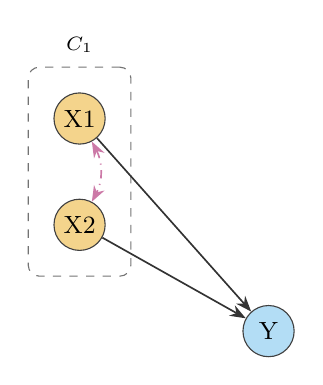
\begin{tikzpicture}
  \node[mannode] (nX1) at (0.00,0.00) {X1};
  \node[mannode] (nX2) at (0.00,-1.35) {X2};
  \node[tgtnode] (nY) at (2.40,-2.70) {Y};
  \draw[diredge] (nX1) -- (nY);
  \draw[diredge] (nX2) -- (nY);
  \draw[biintra] (nX1) to[bend left=28] (nX2);
  \begin{scope}[on background layer]
    \node[clbox,fit=(nX1)(nX2),label={[label distance=0.5mm]above:{\scriptsize$C_{1}$}}] {};
  \end{scope}
\end{tikzpicture}}\hfill
\adjustbox{max width=0.38\linewidth,valign=c}{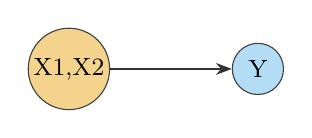
\begin{tikzpicture}
  \node[tgtnode] (nY) at (2.40,0.00) {Y};
  \node[mannode] (nX1X2) at (0.00,0.00) {X1,X2};
  \draw[diredge] (nX1X2) -- (nY);
\end{tikzpicture}}
\caption{\textbf{ParallelParent (MinimalBench, Exp.\ A).} Fine DAG with coarse partition (left) and quotient C-DAG (right), in the convention of Fig.~\ref{fig:motivating}: manipulable variables orange, target blue, dash-dotted latent confounding; dashed boxes are the manipulable clusters. The intra-cluster $X_1\leftrightarrow X_2$ disappears in the quotient; deleting $X_1\to Y$ leaves $C_1\to Y$ alive through $X_2\to Y$ (quotient-redundant).}
\label{fig:dag-parallelparent}
\end{figure}

\begin{figure}[t]\centering
\adjustbox{max width=0.58\linewidth,valign=c}{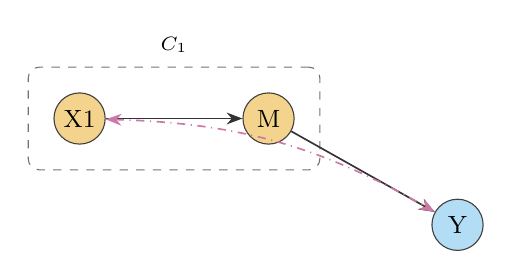
\begin{tikzpicture}
  \node[mannode] (nX1) at (0.00,0.00) {X1};
  \node[mannode] (nM) at (2.40,0.00) {M};
  \node[tgtnode] (nY) at (4.80,-1.35) {Y};
  \draw[diredge] (nX1) -- (nM);
  \draw[diredge] (nM) -- (nY);
  \draw[bicross] (nX1) to[bend left=14] (nY);
  \begin{scope}[on background layer]
    \node[clbox,fit=(nX1)(nM),label={[label distance=0.5mm]above:{\scriptsize$C_{1}$}}] {};
  \end{scope}
\end{tikzpicture}}\hfill
\adjustbox{max width=0.38\linewidth,valign=c}{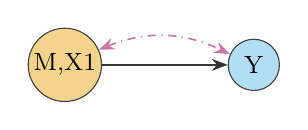
\begin{tikzpicture}
  \node[mannode] (nMX1) at (0.00,0.00) {M,X1};
  \node[tgtnode] (nY) at (2.40,0.00) {Y};
  \draw[diredge] (nMX1) -- (nY);
  \draw[bicross] (nMX1) to[bend left=24] (nY);
\end{tikzpicture}}
\caption{\textbf{FrontDoor (MinimalBench, Exp.\ B).} Fine DAG with coarse partition (left) and quotient C-DAG (right), in the convention of Fig.~\ref{fig:motivating}: manipulable variables orange, target blue, dash-dotted latent confounding; dashed boxes are the manipulable clusters. The quotient is a bow ($C_1\to Y$, $C_1\leftrightarrow Y$): the cluster arm runs on the uninformative prior tier in every condition, so the assumed intra-cluster $X_1\leftrightarrow M$ cannot change it.}
\label{fig:dag-frontdoor}
\end{figure}

\begin{figure}[t]\centering
\adjustbox{max width=0.58\linewidth,valign=c}{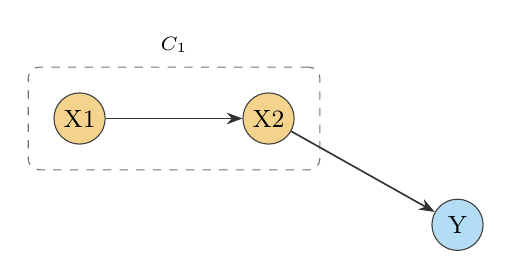
\begin{tikzpicture}
  \node[mannode] (nX1) at (0.00,0.00) {X1};
  \node[mannode] (nX2) at (2.40,0.00) {X2};
  \node[tgtnode] (nY) at (4.80,-1.35) {Y};
  \draw[diredge] (nX1) -- (nX2);
  \draw[diredge] (nX2) -- (nY);
  \begin{scope}[on background layer]
    \node[clbox,fit=(nX1)(nX2),label={[label distance=0.5mm]above:{\scriptsize$C_{1}$}}] {};
  \end{scope}
\end{tikzpicture}}\hfill
\adjustbox{max width=0.38\linewidth,valign=c}{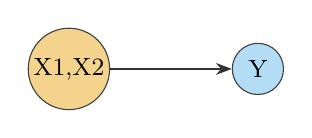
\begin{tikzpicture}
  \node[tgtnode] (nY) at (2.40,0.00) {Y};
  \node[mannode] (nX1X2) at (0.00,0.00) {X1,X2};
  \draw[diredge] (nX1X2) -- (nY);
\end{tikzpicture}}
\caption{\textbf{MediatedChain (MinimalBench, Exp.\ C).} Fine DAG with coarse partition (left) and quotient C-DAG (right), in the convention of Fig.~\ref{fig:motivating}: manipulable variables orange, target blue, dash-dotted latent confounding; dashed boxes are the manipulable clusters. The policy box restricts $D(X_2)$ to $[-2,2]$; the fine optimum $\doo(X_1{=}2)$ drives $X_2$ to $4$, outside the box.}
\label{fig:dag-mediatedchain}
\end{figure}

\begin{figure}[t]\centering
\adjustbox{max width=0.58\linewidth,valign=c}{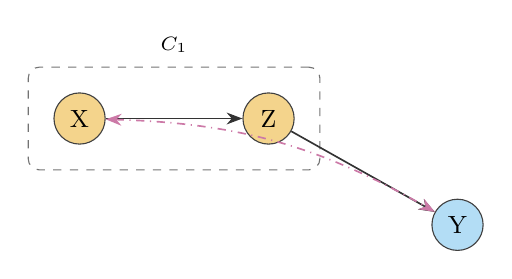
\begin{tikzpicture}
  \node[mannode] (nX) at (0.00,0.00) {X};
  \node[mannode] (nZ) at (2.40,0.00) {Z};
  \node[tgtnode] (nY) at (4.80,-1.35) {Y};
  \draw[diredge] (nX) -- (nZ);
  \draw[diredge] (nZ) -- (nY);
  \draw[bicross] (nX) to[bend left=14] (nY);
  \begin{scope}[on background layer]
    \node[clbox,fit=(nX)(nZ),label={[label distance=0.5mm]above:{\scriptsize$C_{1}$}}] {};
  \end{scope}
\end{tikzpicture}}\hfill
\adjustbox{max width=0.38\linewidth,valign=c}{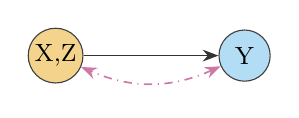
\begin{tikzpicture}
  \node[tgtnode] (nY) at (2.40,0.00) {Y};
  \node[mannode] (nXZ) at (0.00,0.00) {X,Z};
  \draw[diredge] (nXZ) -- (nY);
  \draw[bicross] (nY) to[bend left=24] (nXZ);
\end{tikzpicture}}
\caption{\textbf{ToyGraph (CBO family).} Fine DAG with coarse partition (left) and quotient C-DAG (right), in the convention of Fig.~\ref{fig:motivating}: manipulable variables orange, target blue, dash-dotted latent confounding; dashed boxes are the manipulable clusters. The quotient is a bow ($C_1\to Y$, $C_1\leftrightarrow Y$): $\doo(C_1)$ is not identifiable from the C-DAG, so the arm runs on the uninformative prior tier.}
\label{fig:dag-toy}
\end{figure}

\begin{figure}[t]\centering
\adjustbox{max width=0.58\linewidth,valign=c}{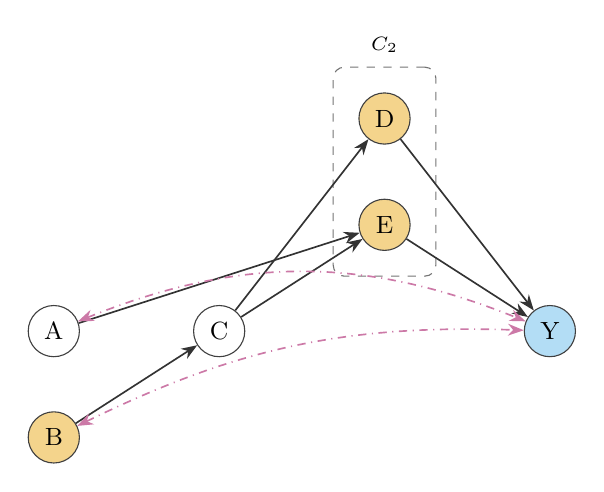
\begin{tikzpicture}
  \node[obsnode] (nA) at (0.00,-2.70) {A};
  \node[mannode] (nB) at (0.00,-4.05) {B};
  \node[obsnode] (nC) at (2.10,-2.70) {C};
  \node[mannode] (nD) at (4.20,0.00) {D};
  \node[mannode] (nE) at (4.20,-1.35) {E};
  \node[tgtnode] (nY) at (6.30,-2.70) {Y};
  \draw[diredge] (nB) -- (nC);
  \draw[diredge] (nC) -- (nD);
  \draw[diredge] (nA) -- (nE);
  \draw[diredge] (nC) -- (nE);
  \draw[diredge] (nD) -- (nY);
  \draw[diredge] (nE) -- (nY);
  \draw[bicross] (nB) to[bend left=14] (nY);
  \draw[bicross] (nA) to[bend left=22] (nY);
  \begin{scope}[on background layer]
    \node[clbox,fit=(nD)(nE),label={[label distance=0.5mm]above:{\scriptsize$C_{2}$}}] {};
  \end{scope}
\end{tikzpicture}}\hfill
\adjustbox{max width=0.38\linewidth,valign=c}{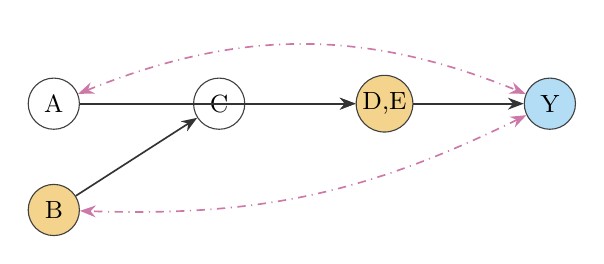
\begin{tikzpicture}
  \node[mannode] (nB) at (0.00,-1.35) {B};
  \node[obsnode] (nC) at (2.10,0.00) {C};
  \node[obsnode] (nA) at (0.00,0.00) {A};
  \node[mannode] (nDE) at (4.20,0.00) {D,E};
  \node[tgtnode] (nY) at (6.30,0.00) {Y};
  \draw[diredge] (nC) -- (nDE);
  \draw[diredge] (nB) -- (nC);
  \draw[diredge] (nA) -- (nDE);
  \draw[diredge] (nDE) -- (nY);
  \draw[bicross] (nY) to[bend left=14] (nB);
  \draw[bicross] (nA) to[bend left=22] (nY);
\end{tikzpicture}}
\caption{\textbf{CompleteGraph (CBO family).} Fine DAG with coarse partition (left) and quotient C-DAG (right), in the convention of Fig.~\ref{fig:motivating}: manipulable variables orange, target blue, dash-dotted latent confounding; dashed boxes are the manipulable clusters.}
\label{fig:dag-complete}
\end{figure}

\begin{figure}[t]\centering
\adjustbox{max width=0.58\linewidth,valign=c}{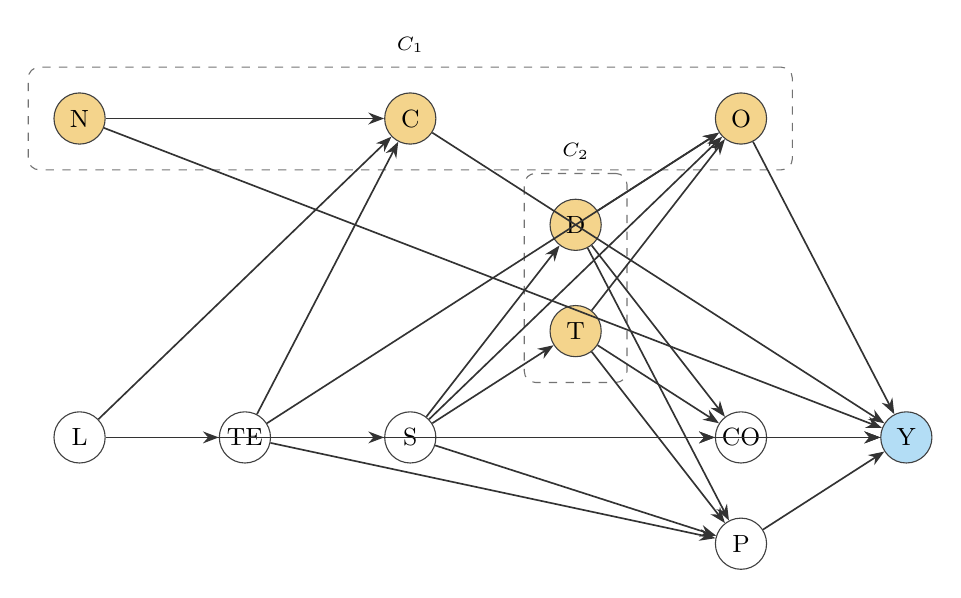
\begin{tikzpicture}
  \node[mannode] (nN) at (0.00,0.00) {N};
  \node[obsnode] (nL) at (0.00,-4.05) {L};
  \node[obsnode] (nTE) at (2.10,-4.05) {TE};
  \node[mannode] (nC) at (4.20,0.00) {C};
  \node[obsnode] (nS) at (4.20,-4.05) {S};
  \node[mannode] (nT) at (6.30,-2.70) {T};
  \node[mannode] (nD) at (6.30,-1.35) {D};
  \node[obsnode] (nP) at (8.40,-5.40) {P};
  \node[mannode] (nO) at (8.40,0.00) {O};
  \node[obsnode] (nCO) at (8.40,-4.05) {CO};
  \node[tgtnode] (nY) at (10.50,-4.05) {Y};
  \draw[diredge] (nL) -- (nTE);
  \draw[diredge] (nL) -- (nC);
  \draw[diredge] (nL) -- (nY);
  \draw[diredge] (nN) -- (nC);
  \draw[diredge] (nN) -- (nY);
  \draw[diredge] (nTE) -- (nC);
  \draw[diredge] (nTE) -- (nS);
  \draw[diredge] (nTE) -- (nP);
  \draw[diredge] (nTE) -- (nO);
  \draw[diredge] (nTE) -- (nCO);
  \draw[diredge] (nTE) -- (nY);
  \draw[diredge] (nS) -- (nT);
  \draw[diredge] (nS) -- (nD);
  \draw[diredge] (nS) -- (nP);
  \draw[diredge] (nS) -- (nO);
  \draw[diredge] (nS) -- (nCO);
  \draw[diredge] (nT) -- (nP);
  \draw[diredge] (nT) -- (nO);
  \draw[diredge] (nT) -- (nCO);
  \draw[diredge] (nD) -- (nP);
  \draw[diredge] (nD) -- (nO);
  \draw[diredge] (nD) -- (nCO);
  \draw[diredge] (nP) -- (nY);
  \draw[diredge] (nO) -- (nY);
  \draw[diredge] (nC) -- (nY);
  \draw[diredge] (nCO) -- (nY);
  \begin{scope}[on background layer]
    \node[clbox,fit=(nC)(nN)(nO),label={[label distance=0.5mm]above:{\scriptsize$C_{1}$}}] {};
  \end{scope}
  \begin{scope}[on background layer]
    \node[clbox,fit=(nD)(nT),label={[label distance=0.5mm]above:{\scriptsize$C_{2}$}}] {};
  \end{scope}
\end{tikzpicture}}\hfill
\adjustbox{max width=0.38\linewidth,valign=c}{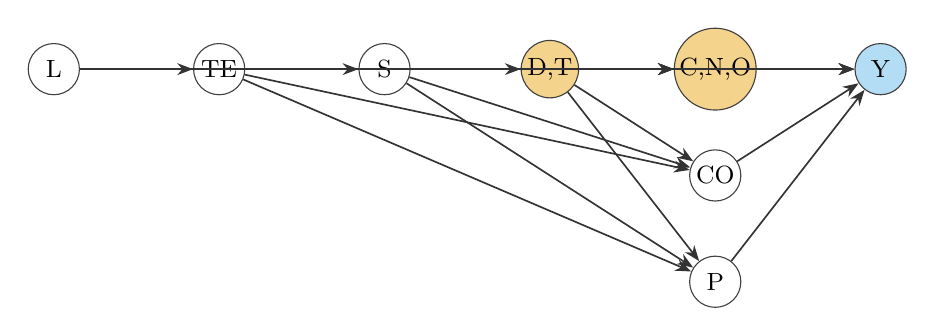
\begin{tikzpicture}
  \node[mannode] (nDT) at (6.30,0.00) {D,T};
  \node[obsnode] (nTE) at (2.10,0.00) {TE};
  \node[mannode] (nCNO) at (8.40,0.00) {C,N,O};
  \node[obsnode] (nS) at (4.20,0.00) {S};
  \node[obsnode] (nCO) at (8.40,-1.35) {CO};
  \node[obsnode] (nP) at (8.40,-2.70) {P};
  \node[obsnode] (nL) at (0.00,0.00) {L};
  \node[tgtnode] (nY) at (10.50,0.00) {Y};
  \draw[diredge] (nL) -- (nY);
  \draw[diredge] (nS) -- (nCNO);
  \draw[diredge] (nCNO) -- (nY);
  \draw[diredge] (nTE) -- (nCNO);
  \draw[diredge] (nTE) -- (nP);
  \draw[diredge] (nDT) -- (nCNO);
  \draw[diredge] (nS) -- (nCO);
  \draw[diredge] (nL) -- (nTE);
  \draw[diredge] (nP) -- (nY);
  \draw[diredge] (nDT) -- (nCO);
  \draw[diredge] (nTE) -- (nCO);
  \draw[diredge] (nDT) -- (nP);
  \draw[diredge] (nL) -- (nCNO);
  \draw[diredge] (nS) -- (nP);
  \draw[diredge] (nCO) -- (nY);
  \draw[diredge] (nS) -- (nDT);
  \draw[diredge] (nTE) -- (nY);
  \draw[diredge] (nTE) -- (nS);
\end{tikzpicture}}
\caption{\textbf{SimplifiedCoralGraph (CBO family).} Fine DAG with coarse partition (left) and quotient C-DAG (right), in the convention of Fig.~\ref{fig:motivating}: manipulable variables orange, target blue, dash-dotted latent confounding; dashed boxes are the manipulable clusters.}
\label{fig:dag-coral}
\end{figure}

\begin{figure}[t]\centering
\adjustbox{max width=0.58\linewidth,valign=c}{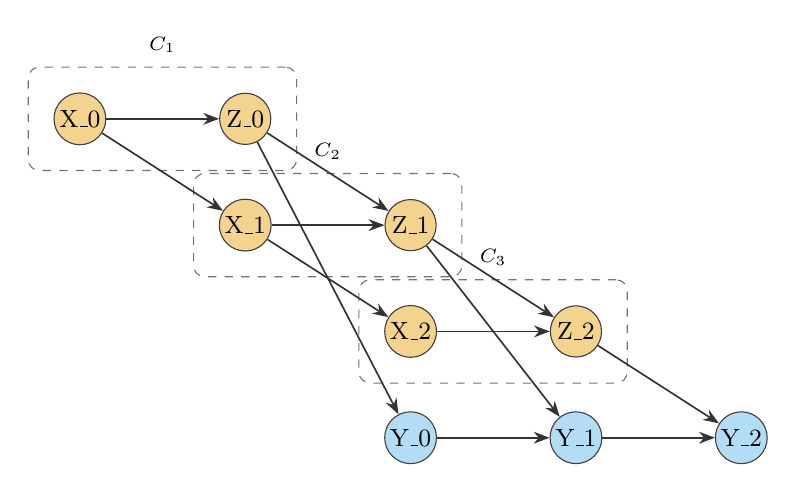
\begin{tikzpicture}
  \node[mannode] (nX0) at (0.00,0.00) {X\_0};
  \node[mannode] (nZ0) at (2.10,0.00) {Z\_0};
  \node[tgtnode] (nY0) at (4.20,-4.05) {Y\_0};
  \node[mannode] (nX1) at (2.10,-1.35) {X\_1};
  \node[mannode] (nZ1) at (4.20,-1.35) {Z\_1};
  \node[tgtnode] (nY1) at (6.30,-4.05) {Y\_1};
  \node[mannode] (nX2) at (4.20,-2.70) {X\_2};
  \node[mannode] (nZ2) at (6.30,-2.70) {Z\_2};
  \node[tgtnode] (nY2) at (8.40,-4.05) {Y\_2};
  \draw[diredge] (nX0) -- (nZ0);
  \draw[diredge] (nZ0) -- (nY0);
  \draw[diredge] (nX1) -- (nZ1);
  \draw[diredge] (nZ1) -- (nY1);
  \draw[diredge] (nX2) -- (nZ2);
  \draw[diredge] (nZ2) -- (nY2);
  \draw[diredge] (nX0) -- (nX1);
  \draw[diredge] (nZ0) -- (nZ1);
  \draw[diredge] (nY0) -- (nY1);
  \draw[diredge] (nX1) -- (nX2);
  \draw[diredge] (nZ1) -- (nZ2);
  \draw[diredge] (nY1) -- (nY2);
  \begin{scope}[on background layer]
    \node[clbox,fit=(nX0)(nZ0),label={[label distance=0.5mm]above:{\scriptsize$C_{1}$}}] {};
  \end{scope}
  \begin{scope}[on background layer]
    \node[clbox,fit=(nX1)(nZ1),label={[label distance=0.5mm]above:{\scriptsize$C_{2}$}}] {};
  \end{scope}
  \begin{scope}[on background layer]
    \node[clbox,fit=(nX2)(nZ2),label={[label distance=0.5mm]above:{\scriptsize$C_{3}$}}] {};
  \end{scope}
\end{tikzpicture}}\hfill
\adjustbox{max width=0.38\linewidth,valign=c}{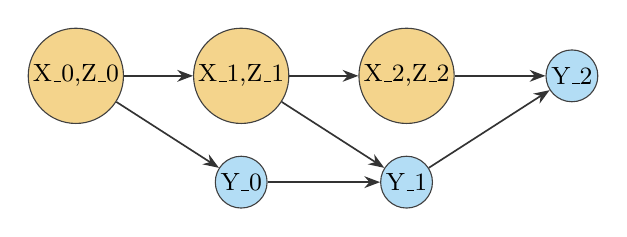
\begin{tikzpicture}
  \node[mannode] (nX0Z0) at (0.00,0.00) {X\_0,Z\_0};
  \node[tgtnode] (nY0) at (2.10,-1.35) {Y\_0};
  \node[mannode] (nX1Z1) at (2.10,0.00) {X\_1,Z\_1};
  \node[tgtnode] (nY1) at (4.20,-1.35) {Y\_1};
  \node[mannode] (nX2Z2) at (4.20,0.00) {X\_2,Z\_2};
  \node[tgtnode] (nY2) at (6.30,0.00) {Y\_2};
  \draw[diredge] (nX0Z0) -- (nY0);
  \draw[diredge] (nX1Z1) -- (nY1);
  \draw[diredge] (nX2Z2) -- (nY2);
  \draw[diredge] (nX0Z0) -- (nX1Z1);
  \draw[diredge] (nY0) -- (nY1);
  \draw[diredge] (nX1Z1) -- (nX2Z2);
  \draw[diredge] (nY1) -- (nY2);
\end{tikzpicture}}
\caption{\textbf{DCBO stat / nonstat (QDCBO family).} Fine DAG with coarse partition (left) and quotient C-DAG (right), in the convention of Fig.~\ref{fig:motivating}: manipulable variables orange, target blue, dash-dotted latent confounding; dashed boxes are the manipulable clusters. Slices $t=0,1,2$; the nonstat setup shares this topology with a change point in the SEM.}
\label{fig:dag-dcbo-stat}
\end{figure}

\begin{figure}[t]\centering
\adjustbox{max width=0.58\linewidth,valign=c}{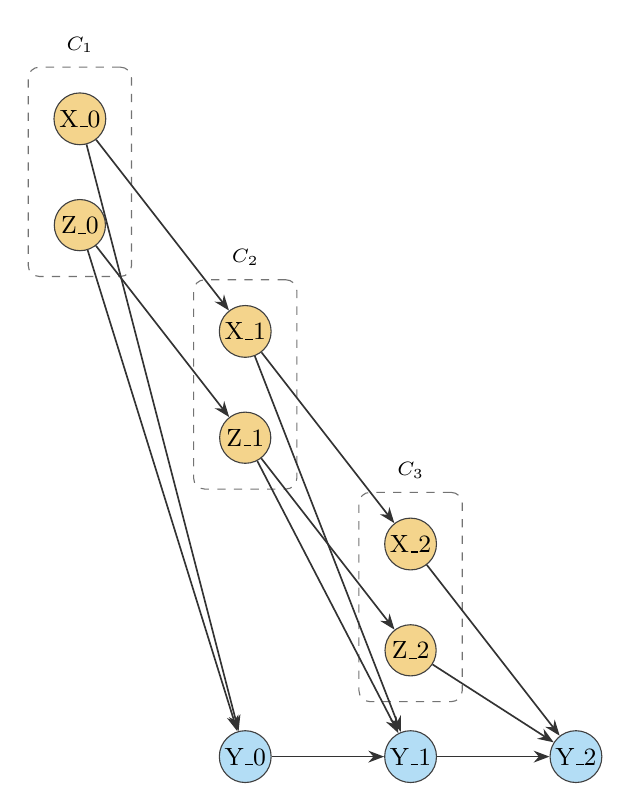
\begin{tikzpicture}
  \node[mannode] (nX0) at (0.00,0.00) {X\_0};
  \node[mannode] (nZ0) at (0.00,-1.35) {Z\_0};
  \node[tgtnode] (nY0) at (2.10,-8.10) {Y\_0};
  \node[mannode] (nX1) at (2.10,-2.70) {X\_1};
  \node[mannode] (nZ1) at (2.10,-4.05) {Z\_1};
  \node[tgtnode] (nY1) at (4.20,-8.10) {Y\_1};
  \node[mannode] (nX2) at (4.20,-5.40) {X\_2};
  \node[mannode] (nZ2) at (4.20,-6.75) {Z\_2};
  \node[tgtnode] (nY2) at (6.30,-8.10) {Y\_2};
  \draw[diredge] (nX0) -- (nY0);
  \draw[diredge] (nZ0) -- (nY0);
  \draw[diredge] (nX1) -- (nY1);
  \draw[diredge] (nZ1) -- (nY1);
  \draw[diredge] (nX2) -- (nY2);
  \draw[diredge] (nZ2) -- (nY2);
  \draw[diredge] (nX0) -- (nX1);
  \draw[diredge] (nZ0) -- (nZ1);
  \draw[diredge] (nY0) -- (nY1);
  \draw[diredge] (nX1) -- (nX2);
  \draw[diredge] (nZ1) -- (nZ2);
  \draw[diredge] (nY1) -- (nY2);
  \begin{scope}[on background layer]
    \node[clbox,fit=(nX0)(nZ0),label={[label distance=0.5mm]above:{\scriptsize$C_{1}$}}] {};
  \end{scope}
  \begin{scope}[on background layer]
    \node[clbox,fit=(nX1)(nZ1),label={[label distance=0.5mm]above:{\scriptsize$C_{2}$}}] {};
  \end{scope}
  \begin{scope}[on background layer]
    \node[clbox,fit=(nX2)(nZ2),label={[label distance=0.5mm]above:{\scriptsize$C_{3}$}}] {};
  \end{scope}
\end{tikzpicture}}\hfill
\adjustbox{max width=0.38\linewidth,valign=c}{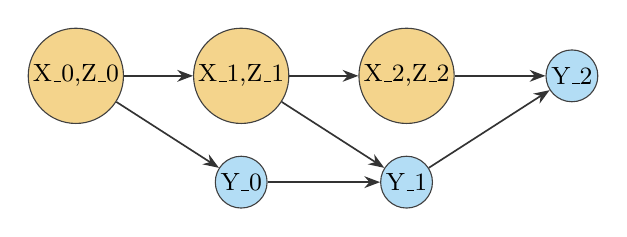
\begin{tikzpicture}
  \node[mannode] (nX0Z0) at (0.00,0.00) {X\_0,Z\_0};
  \node[tgtnode] (nY0) at (2.10,-1.35) {Y\_0};
  \node[mannode] (nX1Z1) at (2.10,0.00) {X\_1,Z\_1};
  \node[tgtnode] (nY1) at (4.20,-1.35) {Y\_1};
  \node[mannode] (nX2Z2) at (4.20,0.00) {X\_2,Z\_2};
  \node[tgtnode] (nY2) at (6.30,0.00) {Y\_2};
  \draw[diredge] (nX0Z0) -- (nY0);
  \draw[diredge] (nX1Z1) -- (nY1);
  \draw[diredge] (nX2Z2) -- (nY2);
  \draw[diredge] (nX0Z0) -- (nX1Z1);
  \draw[diredge] (nY0) -- (nY1);
  \draw[diredge] (nX1Z1) -- (nX2Z2);
  \draw[diredge] (nY1) -- (nY2);
\end{tikzpicture}}
\caption{\textbf{DCBO ind (QDCBO family).} Fine DAG with coarse partition (left) and quotient C-DAG (right), in the convention of Fig.~\ref{fig:motivating}: manipulable variables orange, target blue, dash-dotted latent confounding; dashed boxes are the manipulable clusters.}
\label{fig:dag-dcbo-ind}
\end{figure}

\begin{figure}[t]\centering
\adjustbox{max width=0.58\linewidth,valign=c}{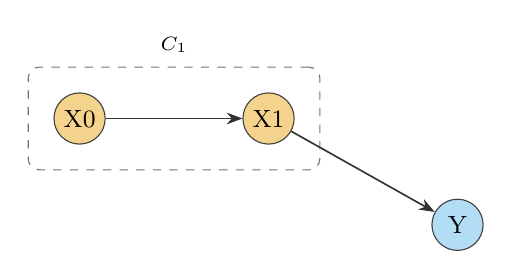
\begin{tikzpicture}
  \node[mannode] (nX0) at (0.00,0.00) {X0};
  \node[mannode] (nX1) at (2.40,0.00) {X1};
  \node[tgtnode] (nY) at (4.80,-1.35) {Y};
  \draw[diredge] (nX0) -- (nX1);
  \draw[diredge] (nX1) -- (nY);
  \begin{scope}[on background layer]
    \node[clbox,fit=(nX0)(nX1),label={[label distance=0.5mm]above:{\scriptsize$C_{1}$}}] {};
  \end{scope}
\end{tikzpicture}}\hfill
\adjustbox{max width=0.38\linewidth,valign=c}{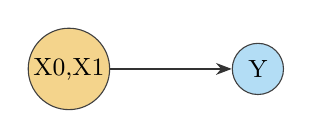
\begin{tikzpicture}
  \node[mannode] (nX0X1) at (0.00,0.00) {X0,X1};
  \node[tgtnode] (nY) at (2.40,0.00) {Y};
  \draw[diredge] (nX0X1) -- (nY);
\end{tikzpicture}}
\caption{\textbf{ToyGraph-M (QMCBO family).} Fine DAG with coarse partition (left) and quotient C-DAG (right), in the convention of Fig.~\ref{fig:motivating}: manipulable variables orange, target blue, dash-dotted latent confounding; dashed boxes are the manipulable clusters.}
\label{fig:dag-mcbo-toygraph-m}
\end{figure}

\begin{figure}[t]\centering
\adjustbox{max width=0.58\linewidth,valign=c}{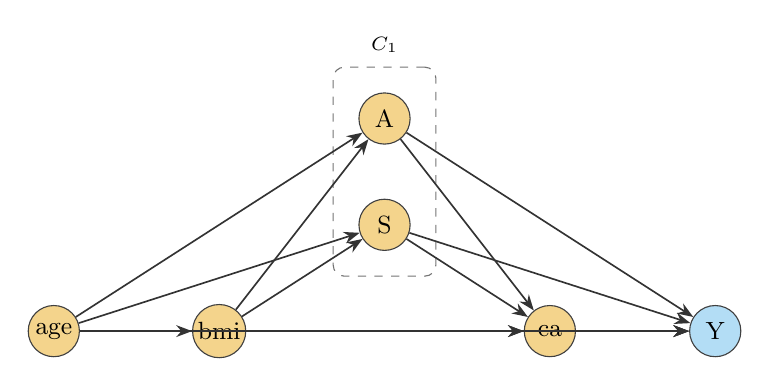
\begin{tikzpicture}
  \node[mannode] (nage) at (0.00,-2.70) {age};
  \node[mannode] (nbmi) at (2.10,-2.70) {bmi};
  \node[mannode] (nA) at (4.20,0.00) {A};
  \node[mannode] (nS) at (4.20,-1.35) {S};
  \node[mannode] (nca) at (6.30,-2.70) {ca};
  \node[tgtnode] (nY) at (8.40,-2.70) {Y};
  \draw[diredge] (nage) -- (nbmi);
  \draw[diredge] (nage) -- (nA);
  \draw[diredge] (nbmi) -- (nA);
  \draw[diredge] (nage) -- (nS);
  \draw[diredge] (nbmi) -- (nS);
  \draw[diredge] (nage) -- (nca);
  \draw[diredge] (nbmi) -- (nca);
  \draw[diredge] (nA) -- (nca);
  \draw[diredge] (nS) -- (nca);
  \draw[diredge] (nage) -- (nY);
  \draw[diredge] (nbmi) -- (nY);
  \draw[diredge] (nA) -- (nY);
  \draw[diredge] (nS) -- (nY);
  \draw[diredge] (nca) -- (nY);
  \begin{scope}[on background layer]
    \node[clbox,fit=(nA)(nS),label={[label distance=0.5mm]above:{\scriptsize$C_{1}$}}] {};
  \end{scope}
\end{tikzpicture}}\hfill
\adjustbox{max width=0.38\linewidth,valign=c}{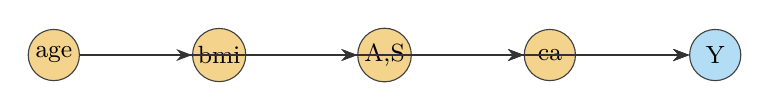
\begin{tikzpicture}
  \node[mannode] (nage) at (0.00,0.00) {age};
  \node[mannode] (nbmi) at (2.10,0.00) {bmi};
  \node[mannode] (nAS) at (4.20,0.00) {A,S};
  \node[mannode] (nca) at (6.30,0.00) {ca};
  \node[tgtnode] (nY) at (8.40,0.00) {Y};
  \draw[diredge] (nage) -- (nbmi);
  \draw[diredge] (nage) -- (nAS);
  \draw[diredge] (nbmi) -- (nAS);
  \draw[diredge] (nage) -- (nca);
  \draw[diredge] (nbmi) -- (nca);
  \draw[diredge] (nAS) -- (nca);
  \draw[diredge] (nage) -- (nY);
  \draw[diredge] (nbmi) -- (nY);
  \draw[diredge] (nAS) -- (nY);
  \draw[diredge] (nca) -- (nY);
\end{tikzpicture}}
\caption{\textbf{PSAGraph (QMCBO family).} Fine DAG with coarse partition (left) and quotient C-DAG (right), in the convention of Fig.~\ref{fig:motivating}: manipulable variables orange, target blue, dash-dotted latent confounding; dashed boxes are the manipulable clusters.}
\label{fig:dag-mcbo-psagraph}
\end{figure}


\endgroup
\clearpage

\end{document}
